\documentclass[a4paper,12pt,oneside]{book}
\usepackage[italian]{babel}
\usepackage{graphicx}%per le immagini
\usepackage{fancyhdr}
\usepackage[font = scriptsize, bf]{caption}
\usepackage[utf8x]{inputenc}
\usepackage[parfill]{parskip}
\usepackage{amsmath, amssymb}
\usepackage{moreverb}
\usepackage{algorithm}
\usepackage{algpseudocode}
\usepackage[usenames,dvipsnames]{color}
\usepackage[swapnames]{frontespizio}
\usepackage{url}
\usepackage{setspace}
\usepackage{eqparbox,array}
%\usepackage[subfigure]{tocloft}
\usepackage{amsthm}
\usepackage{amsmath}
\usepackage{url} % per scrivere gli indirizzi Internet
\usepackage{hyperref}
\usepackage{amsmath}
\usepackage{wrapfig}
\usepackage{caption}
\usepackage{subcaption}
%\newcommand{\algorithmiccomment}[1]{  //\emph{\textcolor{Gray}{#1}}}


% Sistema i margini per lasciare più spazio nella zona di rilegatura
\addtolength{\oddsidemargin}{+1,0cm} 
\addtolength{\evensidemargin}{+1,0cm} 
\onehalfspacing

% Imposta lo stile della prima pagina del capitolo
\fancypagestyle{plain}
{
    \fancyhead{}
    \fancyfoot[LE,RO]{\thepage}
    \renewcommand{\headrulewidth}{0pt}
}

\DeclareMathOperator*{\argmax}{arg\,max}
\newcommand{\compInterfacciaDB}{Data Interface}
\newcommand{\compLoader}{Loader}
\newcommand{\compMatrix}{Matrix Creator}
\newcommand{\compTermsSel}{Terms Selector}
\newcommand{\compPosition}{Position Calculator}
\newcommand{\compClustering}{Clustering Component}
\newcommand{\compEvolution}{Evolution Discoverer}

\hyphenation{ti-me-win-dow}

\graphicspath{{./immagini/}}


\begin{document}

\theoremstyle{definition}
\newtheorem{definizione}{definizione}
\newtheorem{teorema}{Teorema}
% Imposta lo stile di intestazione e piè di pagina della parte iniziale
	\pagestyle{fancy}
	\fancyfoot{}
	\fancyfoot[LE,RO]{\thepage}
	\fancyhead{}
	\renewcommand{\headrulewidth}{0pt}
	\headheight = 15pt


	% frontespizio
	\begin{frontespizio}
		\Universita{Bari - ``Aldo Moro''}
		\Logo[3.5cm]{logo_uni}
		\Facolta{Scienze MM.FF.NN.}
		\Corso{Informatica}
		\Annoaccademico{2014-2015}
		\Titoletto{Tesi di laurea\\in\\Basi di conoscenza e Data Mining}
		\Titolo{TITOLO TESI}
		\Candidato[573394]{Rocco Caruso}
		\NCandidato{Laureando}
		\Relatore{Chiar.mo Prof. Michelangelo Ceci}
		\Relatore{Chiar.mo Prof. Donato Malerba}
		\Correlatore{Dott.ssa Fabiana Lanotte}
		\Correlatore{Dott.    Roberto Corizzo}
		\Margini{3cm}{2cm}{2cm}{2cm}
	\end{frontespizio}
	\frontmatter
	
	% dedica
	\null\vspace{\stretch{1}}
		\begin{flushright}
			\emph{Ahi mè ...}
		\end{flushright}
	\vspace{\stretch{2}}\null
	
	% indice
	\tableofcontents
	\listoftables
	\listoffigures
	\newpage
	\color{white}
	a
	\color{black}
%******************************************************************
% Materiale iniziale
%******************************************************************
%% !TEX encoding = UTF-8
% !TEX TS-program = pdflatex
% !TEX root = ../Tesi.tex
% !TEX spellcheck = it-IT

%*******************************************************
% Frontespizio
%*******************************************************
\begin{frontespizio}
\Preambolo{\usepackage{iwona}} % riga da commentare se non si carica ArsClassica

\Universita{Bologna}
\Logo{Sigillo}
\Facolta{Teologia}
\Corso{Belle Lettere}
\Annoaccademico{2011--2012}
\Titoletto{Tesi di laurea magistrale}
\Titolo{La mia tesi: \\ la prova ontologica \\ dell'esistenza di Dio}
\Sottotitolo{Alcune considerazioni mutevoli}
\Candidato[AB123456]{Lorenzo Pantieri}
\Relatore{Enrico Gregorio}
\Relatore{Claudio Beccari}
\Correlatore{Tommaso Gordini}
\Correlatore{Ivan Valbusa}
\end{frontespizio}





%*******************************************************
% Frontespizio alternativo
%*******************************************************
%\begin{titlepage}
%\pdfbookmark{Frontespizio}{Frontespizio}
%\changetext{}{}{}{((\paperwidth - \textwidth) / 2) - \oddsidemargin - \hoffset - 1in}{}
%\null\vfill
%\begin{center}
%\large
%\sffamily
%\bigskip

%{\LARGE\myName} \\

%\bigskip

%{\Huge\myTitle \\
%}

%\bigskip
    
%\vspace{9cm}

%\begin{tabular}{cc}
%\parbox{0.3\textwidth}{\includegraphics[width=2.5cm]{Sigillo}}
%&
%\parbox{0.7\textwidth}{{\Large\myDegree} \\ 

%					{\normalsize
%					Relatore: \myProf \\
%%					Co-relatore: \myOtherProf \\
%					
%					\myUni \\
%					\myFaculty \\
%					\myDepartment \\
%					\myTime}}
%			\end{tabular}
%\end{center}
%\vfill
%\end{titlepage}







%% !TEX encoding = UTF-8
% !TEX TS-program = pdflatex
% !TEX root = ../Tesi.tex
% !TEX spellcheck = it-IT

%*******************************************************
% Colophon
%*******************************************************
\clearpage
\phantomsection
\thispagestyle{empty}

\hfill

\vfill

%\noindent\myName: \textit{\myTitle,}
%\myDegree,
%\textcopyright\ \MakeTextLowercase{\myTime}.

\lipsum[2]
%% !TEX encoding = UTF-8
% !TEX TS-program = pdflatex
% !TEX root = ../Tesi.tex
% !TEX spellcheck = it-IT

%*******************************************************
% Dedica
%*******************************************************
\cleardoublepage
\phantomsection
\thispagestyle{empty}
\pdfbookmark{Dedica}{Dedica}

\vspace*{3cm}

\begin{center}
Lorem ipsum dolor sit amet, consectetuer adipiscing elit. \\ \medskip
--- Oscar Wilde    
\end{center}

\medskip

\begin{center}
Dedicato a tutti gli appassionati di \LaTeX.
\end{center}
%% !TEX encoding = UTF-8
% !TEX TS-program = pdflatex
% !TEX root = ../Tesi.tex
% !TEX spellcheck = it-IT

%*******************************************************
% Indici
%*******************************************************
\cleardoublepage
\pdfbookmark{\contentsname}{tableofcontents}
\setcounter{tocdepth}{2}
\tableofcontents
\markboth{\spacedlowsmallcaps{\contentsname}}{\spacedlowsmallcaps{\contentsname}} 
\clearpage

\begingroup 
    \let\clearpage\relax
    \let\cleardoublepage\relax
    \let\cleardoublepage\relax
    %*******************************************************
    % Elenco delle figure
    %*******************************************************    
    \phantomsection
    \pdfbookmark{\listfigurename}{lof}
    \listoffigures

    \vspace*{8ex}

    %*******************************************************
    % Elenco delle tabelle
    %*******************************************************
    \phantomsection
    \pdfbookmark{\listtablename}{lot}
    \listoftables
        
    \vspace*{8ex}
       
\endgroup

\cleardoublepage

%% !TEX encoding = UTF-8
% !TEX TS-program = pdflatex
% !TEX root = ../Tesi.tex
% !TEX spellcheck = it-IT

%*******************************************************
% Sommario+Abstract
%*******************************************************
\cleardoublepage
\phantomsection
\pdfbookmark{Sommario}{Sommario}
\begingroup
\let\clearpage\relax
\let\cleardoublepage\relax
\let\cleardoublepage\relax

\chapter*{Sommario}

\lipsum[1]

\vfill

\selectlanguage{english}
\pdfbookmark{Abstract}{Abstract}
\chapter*{Abstract}

\lipsum[2]

\selectlanguage{italian}

\endgroup			

\vfill


%% !TEX encoding = UTF-8
% !TEX TS-program = pdflatex
% !TEX root = ../Tesi.tex
% !TEX spellcheck = it-IT

%*******************************************************
% Ringraziamenti
%*******************************************************
\cleardoublepage
\phantomsection
\pdfbookmark{Ringraziamenti}{ringraziamenti}

\begin{flushright}{\slshape    
	Lorem ipsum dolor sit amet, consectetuer adipiscing elit. \\
	Ut purus elit, vestibulum ut, placerat ac, adipiscing vitae, felis. \\
	Curabitur dictum gravida mauris.} \\ \medskip
    --- Donald Ervin Knuth
\end{flushright}


\bigskip

\begingroup
\let\clearpage\relax
\let\cleardoublepage\relax
\let\cleardoublepage\relax

\chapter*{Ringraziamenti}

\lipsum[1]

\bigskip
 
\noindent\textit{\myLocation, \MakeTextLowercase{\myTime}}
\hfill L.~P.

\endgroup
% !TEX encoding = UTF-8
% !TEX TS-program = pdflatex
% !TEX root = ../tesi.tex
% !TEX spellcheck = it-IT

%*******************************************************
% Introduzione
%*******************************************************
\cleardoublepage
\chapter*{Introduzione}
Twitter è ad oggi il servizio di micro-blogging più utilizzato in assoluto, con circa 284 milioni di utenti attivi al mese, ogni giorno vengono prodotti oltre 500 milioni di tweets. Gli utenti di Twitter, possono pubblicare degli status, o \emph{tweets}, non  più lunghi di 140 caratteri. Se questo vincolo da una parte costituisce un forte limite, dall'altro rappresenta una delle caratteristiche fondamentali di Twitter: \emph{l'immediatezza}. Questo limite costringe gli utenti ad produrre messaggi molto sintetizzati, quasi come slogan, che quindi sono più facili da diffondere. Grazie a queste caratteristiche, qualsiasi persona che assiste o è coinvolta in un \emph{evento}, è in grado di diffondere informazioni in \emph{real-time}.
Talvolta, i tweets (Twitter microblog posts) diffondono notizie anche più velocemente dei media tradizionali (come la morte di Micheal Jackson \footnote{ttp://www.dailymail.co.uk/sciencetech/article-1195651/How-Michael-Jacksons-death-shut-
Twitter-overwhelmed-Google–killed-Jeff-Goldblum.html}).
Bisogna però sottolineare che questi tweet che possono riflettere eventi, rappresentano solo una piccola percentuale di tutti i tweet prodotti. La maggior parte infatti, è costituita da status personali, messaggi anche privi di senso, spam. Risulta quindi necessario un sistema che sia capace di scoprire \lq\lq eventi\rq\rq o \lq\lq topics\rq\rq   da questo flusso di dati.  Affinché questi eventi abbiano una qualche utilità, è altresì necessario, che siano  rilevati con una bassa latenza. I classici algoritmi di Data Mining, non riescono a scalare all'aumentare della mole dei dati . Questo lavoro di tesi ha l'obiettivo di applicare algoritmi di data Mining per la scoperta di eventi, attraverso un'architettura di calcolo distribuita: Apache SPARK. 

Scoprire nuovi eventi o topics da Twitter, non è affatto un task banale sia 
sia la mole dei dati (oltre 400 milioni di tweet giornalmente), che per la natura stessa dei tweets. Se da un lato il limite a 140 caratteri ne rende più semplice la diffusione on-line, dall'altro complica ulteriormente il task, poiché gli utenti spesso,proprio a causa di tale limite,ricorrono a slang, vocaboli OOV\footnote{Out Of Vocabolary} o emoticons.
\section*{Twitter}
Twitter è ad oggi il servizio di "microblogging" più diffuso e con il più alto tasso di crescita.  Negli anni la sua popolarità crescente ha anche attirato anche un alto numero di ricercatori, come si può notare dall'alto numero di articoli riguardanti Twitter che sono stati pubblicati in numerosi campi di ricerca.
Sebbene il termine  “microblog” spesso possa indurre intendere tale servizio come una versione "micro" di un blog, sono due due media molto diversi fra loro \cite{export:69500}. I blog infatti sono progettati, principalmente per permettere ad utenti, di fornire commenti e opinioni su topic di cui sono esperti, gli autori devono anche garantire una certa validità dei contenuti. Dall'altra parte, i microblog, come Twitter, sono invece pensati per permettere di condividere opinioni, news, ma in maniera molto concisa (max 140 caratteri) proprio per far sì che si abbia una  diffusione tempestiva delle informazioni. Proprio grazie a questa caratteristica, i tweets possono essere pubblicati mediante dispositivi mobili, consentendo a chiunque sia testimone di un qualsiasi evento di diffondere la notizia in real-time. Twitter inoltre è anche un servizio di social networking, ogni utente può ricevere gli aggiornamenti ("follow")  di altri utenti senza previa approvazione. Questa relazione è asimmetrica e può essere concettualizzata come una Directed social network o \emph{follower network} 
\subsection*{Twitter come fonte di informazione}
Molte notizie sono state diffuse su Twitter anche prima della diffusione sui media classici. Uno degli esempi più significati è stato rappresentato dalla notizia della di Michael Jackson del 2009. Alle 2:26pm
del 24 Giungo 2009, la notizia trapelò su Twitter e fu diffusa in una maniera così virale che che Google la identificò come un attacco hacker.t . La validità della notizia fù verificata da Google solo 25 minuti dopo,   solo allora i media mainstream iniziarono a far diffondere la notizia \footnote{ttp://www.dailymail.co.uk/sciencetech/article-1195651/How-Michael-Jacksons-death-shut-
Twitter-overwhelmed-Google–killed-Jeff-Goldblum.html}.Anche nel caso del terremoto in Abruzzo del 6 aprile 2009, gli utenti Twitter hanno segnalato la notizia prima dei media tradizionali. 

%\pagestyle{scrheadings} 
%\cleardoublepage
%******************************************************************
% Materiale principale
%******************************************************************


% capitoli
	% frontespizio
	
	\frontmatter	
	\mainmatter

	% Imposta lo stile di intestazione e piè di pagina dei capitoli
	\fancyfoot{}
	\fancyhead{}
	\fancyhead[LE,RO]{\slshape \leftmark}
	\fancyfoot[LE,RO]{\thepage}
	\renewcommand{\headrulewidth}{1pt}
	\renewcommand{\chaptermark}[1]{%
	\markboth{\thechapter.\ #1}{}}

\label{cap:capitoloIntro}
% !TEX encoding = UTF-8
% !TEX TS-program = pdflatex
% !TEX root = ../tesi.tex
% !TEX spellcheck = it-IT

%************************************************
\chapter{Introduzione}
%************************************************
Scoprire nuovi eventi o topics da Twitter, non è affatto un task banale sia 
sia la mole dei dati (oltre 400 milioni di tweet giornalmente), che per la natura stessa dei tweets. Se da un lato il limite a 140 caratteri ne rende più semplice la diffusione on-line, dall'altro complica ulteriormente il task, poiché gli utenti spesso,proprio a causa di tale limite,ricorrono a slang, vocaboli OOV\footnote{Out Of Vocabolary} o emoticons.
\section{Twitter}
Twitter è ad oggi il servizio di "microblogging" più diffuso e con il più alto tasso di crescita.  Negli anni la sua popolarità crescente ha anche attirato anche un alto numero di ricercatori, come si può notare dall'alto numero di articoli riguardanti Twitter che sono stati pubblicati in numerosi campi di ricerca.
Sebbene il termine  “microblog” spesso possa indurre intendere tale servizio come una versione "micro" di un blog, sono due due media molto diversi fra loro \cite{export:69500}. I blog infatti sono progettati, principalmente per permettere ad utenti, di fornire commenti e opinioni su topic di cui sono esperti, gli autori devono anche garantire una certa validità dei contenuti. Dall'altra parte, i microblog, come Twitter, sono invece pensati per permettere di condividere opinioni, news, ma in maniera molto concisa (max 140 caratteri) proprio per far sì che si abbia una  diffusione tempestiva delle informazioni. Proprio grazie a questa caratteristica, i tweets possono essere pubblicati mediante dispositivi mobili, consentendo a chiunque sia testimone di un qualsiasi evento di diffondere la notizia in real-time. Twitter inoltre è anche un servizio di social networking, ogni utente può ricevere gli aggiornamenti ("follow")  di altri utenti senza previa approvazione. Questa relazione è asimmetrica e può essere concettualizzata come una Directed social network o \emph{follower network} 
\subsection{Twitter come fonte di informazione}
Molte notizie sono state diffuse su Twitter anche prima della diffusione sui media classici. Uno degli esempi più significati è stato rappresentato dalla notizia della di Michael Jackson del 2009. Alle 2:26pm
del 24 Giungo 2009, la notizia trapelò su Twitter e fu diffusa in una maniera così virale che che Google la identificò come un attacco hacker.t . La validità della notizia fù verificata da Google solo 25 minuti dopo,   solo allora i media mainstream iniziarono a far diffondere la notizia \footnote{ttp://www.dailymail.co.uk/sciencetech/article-1195651/How-Michael-Jacksons-death-shut-
Twitter-overwhelmed-Google–killed-Jeff-Goldblum.html}.Anche nel caso del terremoto in Abruzzo del 6 aprile 2009, gli utenti Twitter hanno segnalato la notizia prima dei media tradizionali. 
\section{Big Data}
Sebbene oggigiorno il termine \lq\lq big data\rq\rq sia molto in voga, la sua definizione è ancora piuttosto vaga. Alcuni definizioni fanno riferimento al volume dei dati, altre  invece fanno riferimento alla ricchezza dei dati. Per altri, i \lq\lq big data\rq\rq sono   quei dati troppo grandi per gli standard tradizionali, ovvero quando il volume dei dati supera petabytes o zettabytes. Altri ancora intendono per big data, quei dati che riescono ad esprimere più sfaccettature delle stesse entità che rappresentano, che se fossero memorizzati nei classici database relazionali (RDBMS) avrebbero migliaia di colonne. 
L'aggettivo \lq\lq big\lq\lq non si riferisce soltanto al volume dei dati, ma anche alla loro complessità. Esistono infatti, molti piccoli datasets che  sono considerati big data che non richiedono molo spazio di memorizzazione, ma hanno una complessità intrinseca molto alta. Allo stesso tempo, datasets che richiedono molto spazio di memorizzazione possono non essere abbastanza complessi, da essere considerati Big data. Il solo volume dei dati, quindi non basta a definire questi big-data. Una definizione molto diffusa è quella delle tre \emph{V}, dove, oltre al volume dei dati, si considera anche la Velocità e la Varietà .
Per Velocità si intende che i dati sono generati con un'elevata frequenza.
La Varietà si riferisce al fatto che i dati possono essere  strutturati, semi strutturati o non strutturati affatto : dati transazionali, video, audio testo file di log.
In aggiunta a queste tre V, talvolta viene aggiunta una quarta alla definizione: \emph{Veridicità}.
La veridicità è un indicazione dell'integrità di questi dati e si riferisce al livello di trust in questi dati stessi, affinché si possano utilizzare nei processi decisionali
Analizzare questi big-data può permettere  di prendere decisioni in maniera più oculata e molto più velocemente, usando dati che in passato erano inaccessibili o inutilizzabili.
Per tali ragioni, i classici database relazionali non riescono a gestire facilmente questi dati.
\section{Hadoop}
Hadoop è stato uno dei primi sistemi open-source più popolari per processare i big data.
\'E un sistema scalabile e fault-tolerant che consente di processare grandi dataset attraverso un cluster di server.  


\begin{figure}[h]
\centering
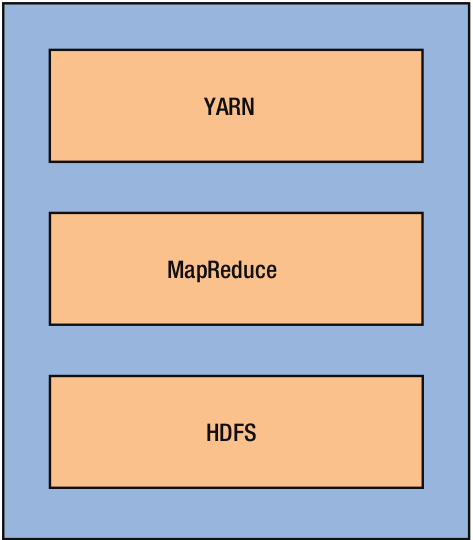
\includegraphics[width=0.4\textwidth]{hadoopCompo.png}
\caption{componenti principali di Hadooop}
\label{fig:hadoopComponets}
\end{figure} 
 
Uno dei fattori di successo di Hadoop è il basso costo. Hadoop è un sistema open-source che può essere eseguito su un cluster di commodity\footnote{hardware non dedicato di basso costo} hardware. Riesce cioè a garantire facilmente una scalabilità orizzontale aggiungendo al cluster, dei server poco costosi. Inoltre, riesce a garantire, via software la tolleranza ai guasti: assume che prima o poi vi saranno dei guasti e li gestisce in maniera trasparente. Uno sviluppatore software non dovrà preoccuparsi di gestire questi fault. Consente, cioè, di sviluppare applicazioni distribuite in maniera molto più semplice poiché viene sperata la logica di elaborazione dei dati dalla logica di distribuzione dei dati.
Hadoop è composto da tre componenti principali: un cluster mananger (YARN), un modello di computazione distribuito (Map-reduce) e un file system distribuito (HDFS)



 
 \subsection{Map Reduce}
 MapReduce è il modello di computazione distribuita fornito da Hadoop. Mentre HDFS fornisce un file system distribuito per memorizzare grandi dataset, MapReduce fornisce un framework di computazione che consente di processare grandi dataset in parallelo attraverso un cluster di computer (nodi). Questo modello astrae la computazione distribuita fornendo dei costrutti ad alto livello che consentono di sviluppare facilmente applicazioni distribuite.
 Il framework MapReduce schedula in maniera automatica l'esecuzione di un applicazione su un insieme di macchine in un cluster, prendendosi carico  della gestione della comunicazione fra nodi, del bilanciamento del carico di esecuzione fra i nodi e dei possibili guasti dei nodi.
In questo modo, gli sviluppatori possono concentrarsi sulla logica di processing dei dati tralasciando questi dettagli.

Come suggerisce il nome stesso, questo modello si basa su due funzioni :\emph{map}   e \emph{reduce}. Tutti i carichi di lavoro in un appplicazione MapReduce sono espressi implementando queste due funzioni.
La funzione \emph{map} riceve in input una coppia chiave-valore e restituisce a sua volta una insieme di  coppie chiave valore intermedie. Il framework MapReduce esegue la funzione map per ogni coppia chiave valore presente nel dataset di input. L'output delle funzioni Map, è ordinato e raggruppato in base ai valori di chiave intermedi, e costituirà l'input della funzione Reduce. La funzione \emph{Reduce} aggrega i risultati della funzione map, in base al valore di chiave intermedio.

I dati possono essere sia semi strutturati o non strutturati affatto, non è richiesto che i dati siano conformi ad uno schema rigido predefinito. L'unico requisito è che sia possibile esprimere il dataset in input come una serie di coppie chiave valore.
Il modello MapReduce ha rivoluzionato il modo di processare grandi datasets, offrendo un modello semplice che consente di scrivere programmi che possono essere eseguiti in parallelo su molte macchine. Grazie a questo, Map-Reduce consente di ottenere una scalabilità orizzontale: all'aumentare della dimensione dei dati è possibile aggiungere nuove macchine mantenendo quasi invariato il tempo di esecuzione.
\section{Apache Spark}
Apache Spark \cite{Zaharia:2010:SCC:1863103.1863113} è una framework open-source che consente di processare grandi dataset in maniera distribuita.
Spark può essere considerato come il successore del modello MapReduce di Hadoop, entrambi i framwork sono progettati per poter processare i big data.  Spark mantiene inalterata la scalabilità di MapReduce e la tolleranza ai guasti, e inoltre aggiunge nuove caratteristiche, offrendo inoltre ulteriori vantaggi rispetto a MapReduce. Primo fra questi è la velocità: Spark riesce a processare i dati riducendo  di molto i tempi di latenza (fino a 100 volte), poiché  consente ai nodi di processing di immagazzinare in memoria centrale i risultati intermedi, a differenza di MapReduce, dove invece erano serializzati sul file system.  La velocità può essere talvolta un fattore determinante. Impiegare troppo tempo per processare i dati, rallenta tutto il processo decisionale riducendo il valore stesso dei dati.
La principale astrazione fornita da SPARK sono i \textbf{R}esilent \textbf{D}istributed \textbf{D}ataset (RDD) \cite{Zaharia:2012:RDD:2228298.2228301}, che essenzialmente sono una collezione immutabile e distribuita di oggetti. Questi oggetti sono, suddivisi in più partizioni che  generalmente sono distribuite su più nodi.
Questa astrazione permette agli sviluppatori di materializzare i risultati intermedi della computazione  nella memoria dei vari nodi di processing. Ciò signfica che i prossimi step che vogliono riconsultare questi dati, non li dovranno rielaborare o ricaricare da disco.
Per tale ragione, Spark si presta bene per eseguire in parallelo sia algoritmi altamente iterativi che richiedono di scansionare un dataset di input più volte, come gli algoritmi di machine-leanring.

Questi RDD possono essere creati in due modi: o a partire da dati in un sistema di memorizzazione stabile\footnote{per stabile si intende fault-tolerant} (HDFS, Hive, Cassandra, ) o a partire da altri RDD. Queste operazioni, che creano RDD, sono dette \emph{trasformazioni}.

Spark non materializzare gli RDD dopo ogni operazione, verrà memorizzato per ogni RDD intermedio il suo \emph{lineage} ovvero la sequenza di trasformazioni che lo ha prodotto, a partire da un altro RDD. In tal modo SPARK nel caso vi sia un failure, può rielaborare un RDD in maniera del tutto trasparente.
 
Architetturalmente, Spark è progettato per essere altamente accessibile: offre API per Python, Java, Scala, SQL e R. Inoltre si integra alla perfezione con strumenti di Big Data quali Hadoop (e strumenti che dipendono da esso come HBase, Hive, etc.) e Cassandra.




 
\begin{figure}[htbp]
    \makebox[\textwidth]{
        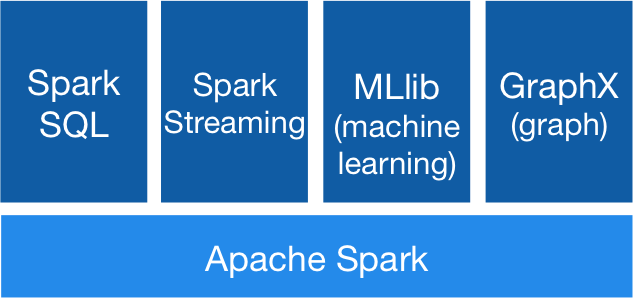
\includegraphics[width=0.7\textwidth]{spark-stack.png}
    }
    \caption{Stack applicativo Apache Spark}
    \label{fig:sparkstack}
\end{figure}




La figura \ref{fig:sparkstack} mostra le principali componenti di Apache Spark:
\begin{itemize}
\item \textbf{Spark Core}: contiene le funzionalità base di Spark fra cui l'astrazione sulla quale si basa l'intero ambiente, i \textit{resilient distributed dataset} (RDD).
\item \textbf{Spark SQL}: contiene le componenti per elaborare e manipolare dati strutturati. Permette l'interrogazione (tramite SQL) di dabatase relazionali, JSON, HIVE (mediante lo Hive Query Language) e file Parquet. 
\item \textbf{Spark Streaming}: componente che permette l'elaborazione di stream di dati.
\item \textbf{MLLib}: contiene algoritmi di Machine Learning per vari tipi di task quali classificazione, regressione, clustering, collaborative filtering, frequent pattern mining, dimensionality reduction, feature extraction e statistica di base.
\item \textbf{GraphX}: libreria per la manipolazione ed estrazione di conoscenza in grafi.
\end{itemize}

\subsection{Modello di esecuzione}
Una applicazione Spark consiste in un processo \textit{driver} e di un insieme di processi \textit{executors} distribuiti sui nodi del cluster.

Fra le responsabilità del driver si annoverano:
\begin{itemize}
\item interazione con l'utente;
\item coordinare e distribuire il flusso di controllo.
\end{itemize}


\begin{figure}[h]
\centering
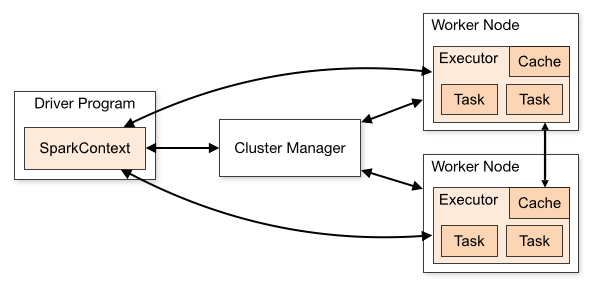
\includegraphics[width=0.8\textwidth]{cluster-ov.png}
\caption{componenti principali di Hadooop}
\label{fig:hadoopComponets}
\end{figure} 
 
I processi "executor" sono responsabili dell'esecuzione dei work in forma di \textit{tasks} e di memorizzare qualsiasi tipo di dato che l'utente sceglie di mantenere in cache. 

In cima al modello di esecuzione vi sono i \textit{jobs}: l'invocazione di una azione all'interno di una applicazione Spark provoca l'esecuzione di uno Spark job in grado di soddisfare la richiesta. Spark esamina il grafo degli RDD dal quale l'zione dipende e produce un piano di esecuzione che inizia computando le risorse (gli RDD) in ordine di dipendenza, culminando con l'RDD che produrrà i risultati dell'azione.
 

Il piano di esecuzione consiste nell'assemblare trasformazioni di jobs in \textit{stages}. Uno stage corrisponde a una collezione di \textit{tasks} che eseguono simultaneamente lo stesso codice su una differenze partizione dei dati: ciascuno stage contiene una sequenza di trasformazioni che possono essere completati senza rimescolare i dati.

Quest'ultimo aspetto inficia fortemente le performance dell'applicazione. Una partizione di dati subisce un processo denominato "shuffling"  quando vengono effettuate trasformazioni \textit{narrow}, ad esempio una \textit{map}.

Il trasferimento dei dati fra i nodi del cluster avviene mediante un meccanismo di serializzazione: dopo questo processo, i dati vengono memorizzati in una cache e trasferiti in rete per uno shuffling. Spark prevede due meccanismi di serializzazione: l'approccio classico (utilizzando le API Java disponibile a partire dall'interfaccia \textit{java.io.Serializable}) e mediante la libreria \textit{Kryo}. Quest'ultima prevede un formato molto più compatto in grado di svolgere le operazioni in maniera più rapida.



\chapter{Stato dell'Arte}
\label{cap:capitolo1}
% !TEX encoding = UTF-8
% !TEX TS-program = pdflatex
% !TEX root = ../tesi.tex
% !TEX spellcheck = it-IT

%************************************************



Il \emph{Micro-blogging} è un nuovo mezzo di comunicazione che permette agli utenti di pubblicare in broadcast  costantemente e in  "real time" brevi contenuti digitali, come testo, link, immagini o video. 
Questi contenuti vengono pubblicati in una rete sociale, in cui ogni utente può generare nuove informazioni, aggiornare informazioni esistenti e condividere o commentare informazioni pubblicate da altri utenti \cite{Java:2007:WWT:1348549.1348556}.  

Negli ultimi anni, questo mezzo di comunicazione ha attirato l'attenzione di una vasta  comunità  di ricercatori e aziende che operano in diversi ambiti.
La popolarità crescente di questi servizi di micro-blogging è dovuta alla loro portabilità, immediatezza e facilità d'uso. Queste caratteristiche consentono agli utenti di interagire istantaneamente e diffondere informazioni.

Virtualmente qualsiasi persona che assiste o è coinvolta in un qualsiasi evento è capace, grazie a questi micro-blog, di diffondere informazioni durante l'accaduto stesso. Ad esempio, durante i recenti conflitti, crisi sociali e manifestazioni\footnote{e.g.: primavera araba, proteste iraniane del 2009, elezioni presidenziali, etc.}, milioni di persone hanno utilizzato sistemi di micro-blogging come Twitter sia per diffondere notizie che per ricevere aggiornamenti sugli ultimi accadimenti.

Twitter è ad oggi il servizio di micro-blogging più utilizzato in assoluto. Con circa 284 milioni di utenti attivi al mese, ogni giorno vengono prodotti oltre 500 milioni di tweets al giorno. Gli utenti di Twitter, possono inviare in broadcast brevi status (\emph{tweets}), non  più lunghi di 140 caratteri,
 ad una rete di utenti (\emph{follower}) attraverso diversi dispositivi (e.g. smartphones, web-app, email, etc.).
 
Se da un lato la dimensionalità dei tweet rappresenta per alcuni utenti un forte limite, dall'altro rappresenta una delle caratteristiche fondamentali di Twitter: \emph{l'immediatezza}. Questo vincolo costringe gli utenti a produrre messaggi molto sintetici, quasi come slogan, che quindi sono più facili da diffondere.

%Inoltre, sebbene  i tweet siano caratterizzati da un contenuto molto ristretto, bisogna considerare che milioni di persone  \emph{twittano}\footnote{http://www.garzantilinguistica.it/ricerca/?q=twittare}  da ogni parte del mondo, a proposito di argomenti più disparati da manifestazioni sportive a crisi globali.
Monitorare e analizzare questo flusso di  contenuti generati degli utenti può portare a scoprire informazioni molto utili. Per esempio, molte aziende utilizzano Twitter sia per pubblicizzare e raccomandare i loro prodotti, che comprendere  le opinioni dei loro clienti riguardo i loro prodotti (o dei loro competitor) .
Inoltre i tweet sono stati analizzati per predire i risultati delle votazioni presidenziali, crimini \cite{Wang2012}, attività terroristiche o eventi. In generale, un evento può essere definito \emph{qualcosa che accade in un luogo e tempo specifico}. 

Diversi lavori in letteratura si sono focalizzati sul problema di estrazione automatica di eventi, dimostrando l'importanza di Twitter come mezzo di comunicazione. Infatti in diverse occasioni si è osservato come le notizie relative ad eventi si diffondano prima e più velocemente delle notizie diffuse sui media tradizionali (come la morte di Micheal Jackson \footnote{ttp://www.dailymail.co.uk/sciencetech/article-1195651/How-Michael-Jacksons-death-shut- Twitter-overwhelmed-Google–killed-Jeff-Goldblum.html}).

Scoprire eventi da Twitter non è un task banale. Infatti, tweet associati ad  eventi, rappresentano solo una piccola percentuale di tutti i tweet prodotti. La maggior parte infatti, è costituita da status personali, messaggi anche privi di senso, spam, etc..   
La maggior parte degli approcci esistenti per l'estrazione automatica di eventi, utilizza la similarità sintattica dei contenuti testuali dei tweets. Queste soluzioni non considerano né il problema della dimensionalità (mole di dati da processare) né tanto meno sfruttano informazioni contestuali quali tempo, luogo o entità coinvolte (e.g. persone o organizzazioni).

La mole dei dati da analizzare e la necessità di estrarre efficientemente risultati rendono il problema dell'estrazione di eventi assimilabile ad un problema  come  "Big Data Analytics".  
Obiettivo di questa tesi, è quello di proporre un sistema scalabile per il task di event detection a partire da twitter, utilizzando un'architettura di calcolo distribuita. Nella soluzione proposta oltre alla classica rappresentazione sintattica dei tweet, sarà adottata una rappresentazione semantica utilizzando la base di conoscenza di DBpedia.


\section{Twitter}
 

Come già detto in precendenza, Twitter è il servizio di micro-blogging più utilizzato in assoluto.

Dalla sua creazione nel 2006, Twitter ottenne rapidamente una popolarità su larga scala 
La funzione principale di Twitter è quella di permettere agli utenti di scrivere e leggere brevi messaggi (max 140 caratteri) noti come \emph{tweets}.

Gli utenti possono \lq\lq twittare\rq\rq attraverso il sito di twitter o tramite applicazioni per smart-phones e persino tramite sms. 
Twitter oltre ad essere un servizio di micro-blogging, è un social-network, ma ha una caratteristica che lo contraddistingue dai più noti come Facebook, Gooogle+ : è 
asimmetrico. Un utente infatti, può seguire (\emph{follow}) lo stream dei tweet generati da un altro utente, senza che quest'ultimo approvi o faccia altrettanto. 
Quando un utente scrive un tweet, questo viene automaticamente viene inviato in broadcast alla rete dei suoi \emph{followers}.

A ciascun utente vengono mostrati i tweet degli utenti che deciso di seguire, sulla sua \emph{timeline}.
La timeline è costituita dallo stream dei tweet ordinati cronologicamente.
Generalmente tutti i tweet sono accessibili pubblicamente, a meno che un utente specifichi un livello di privacy  consentendo che i propri tweets siano visibili solo ai suoi follower.\\

Twitter inoltre permette  varie forme di interazione fra gli utenti.
\'E possibile creare delle vere e proprie conversazioni, grazie al fatto che un utente può scrivere un tweet, in risposta ad un tweet di un altro utente. 	Questa forma di interazione è nota come \emph{reply}.
Un \emph{reply} inizia con il caratattere \emph{@} seguito dall'username dell'utente a cui si sta rispondendo.
Inoltre all'interno di un tweet è possibile menzionare un altro utente facendo precedere il suo username dal carattere  \emph{@}. Questa interazione è anche nota come \emph{@-mention} e rappresenta un caso più generale del \emph{reply} 

Twitter inoltre consente ad un utente di inoltrare o \emph{retwittare} il tweet di qualcun altro, ai propri followers il tweet di un altro utente.


\subsection{Twitter come fonte di informazione}
Molte notizie sono state diffuse su Twitter anche prima della diffusione sui media classici. Uno degli esempi più significati è stato rappresentato dalla notizia della di Michael Jackson del 2009. Alle 2:26pm
del 24 Giungo 2009, la notizia trapelò su Twitter e fu diffusa in una maniera così virale che che Google la identificò come un attacco hacker. La validità della notizia fù verificata da Google solo 25 minuti dopo,   solo allora i media mainstream iniziarono a far diffondere la notizia \footnote{ttp://www.dailymail.co.uk/sciencetech/article-1195651/How-Michael-Jacksons-death-shut-
Twitter-overwhelmed-Google–killed-Jeff-Goldblum.html}.Anche nel caso del terremoto in Abruzzo del 6 aprile 2009, gli utenti Twitter hanno segnalato la notizia prima dei media tradizionali. 
\section{Big Data}
Sebbene oggigiorno il termine \lq\lq big data\rq\rq sia molto in voga, la sua definizione è ancora piuttosto vaga. Alcuni definizioni fanno riferimento al volume dei dati, altre  invece fanno riferimento alla ricchezza dei dati. Per altri, i \lq\lq big data\rq\rq sono   quei dati troppo grandi per gli standard tradizionali, ovvero quando il volume dei dati supera petabytes o zettabytes. Altri ancora intendono per big data, quei dati che riescono ad esprimere più sfaccettature delle stesse entità che rappresentano, che se fossero memorizzati nei classici database relazionali (RDBMS) avrebbero migliaia di colonne. 

L'aggettivo \lq\lq big\rq\rq non si riferisce soltanto al volume dei dati, ma anche alla loro complessità. Esistono infatti, molti   datasets che  sono considerati big data  pur non richiedendo  molto spazio di memorizzazione, poiché hanno una complessità intrinseca molto alta. Allo stesso tempo, datasets che richiedono molto spazio di memorizzazione possono non essere abbastanza complessi, da essere considerati Big data. Il solo volume dei dati, quindi non basta a definire questi big-data. Una definizione molto diffusa è quella delle tre \emph{V}, dove, oltre al volume dei dati, si considera anche la Velocità e la Varietà .
Per Velocità si intende che i dati sono generati con un'elevata frequenza.
La Varietà si riferisce al fatto che i dati possono essere  strutturati, semi strutturati o non strutturati affatto : dati transazionali, video, audio testo file di log.
In aggiunta a queste tre V, talvolta viene aggiunta una quarta alla definizione: \emph{Veridicità}.
La veridicità è un indicazione dell'integrità di questi dati e si riferisce al livello di trust in questi dati stessi, affinché si possano utilizzare nei processi decisionali
Analizzare questi big-data può permettere  di prendere decisioni in maniera più oculata e molto più velocemente, usando dati che in passato erano inaccessibili o inutilizzabili.
Per tali ragioni, i classici database relazionali non riescono a gestire facilmente questi dati.

 Generalmente per processare dataset di grandi dimensioni si possono adottare due strategie.
La prima consiste nell'aumentare la potenza di calcolo della macchina su cui si dovrà elaborare il datasets. Questo strategia è comunemente noto come \emph{\lq\lq scalabilità  verticale\rq\rq}. La seconda strategia  piuttosto che incrementare la potenza di calcolo di una macchina, incrementa il \emph{numero} di macchine per processare il dataset, ed è nota come \emph{\lq\lq scalabilità  orizzontale\rq\rq}.
Negli ultimi anni la seconda strategia ha avuto una forte crescita, divenendo una delle scelte più diffuse per elaborare grandi dataset. Aumentare la potenza di calcolo di una singola macchina è molto costoso, ed inoltre vi è un limite superiore che non è possibile valicare. D'altra parte, la diminuzione dei costi e all'aumento delle prestazioni di workstation, sono stati dei fattori trainanti nella crescita di soluzioni di calcolo distribuito scalabili orizzontalmente. Oggi è possibile raggiungere quasi la stessa potenza di calcolo di un server dedicato (molto costoso), attraverso molte workstation (poco costose). 
Inoltre, distribuire la computazione su più nodi rende molto più difficile gestire l'allocazione dei task. Idealmente quello che si vorrebbe ottenere, è che ogni task di elaborazione sia suddiviso in parti uguali sui vari nodi, in pratica però questa caratteristica è difficile da ottenere.
Questa difficoltà deriva dal fatto che non sempre i dati sono disponibili su tutti i nodi di elaborazione, ma soprattutto dal fatto che non tutte le computazioni sono facilmente suddivisibili in parti uguali.
Bisogna però considerare che, passare ad una soluzione scalabile orizzontalmente pone nuove sfide. Innanzitutto, all'aumentare del numero di nodi ci calcolo, aumenta anche la probabilità che su uno un nodo qualsiasi si abbia un guasto, rendendo molto più difficile assicurare che l'elaborazione dei dati sia \emph{affidabile}.

 \subsection{Hadoop}
Hadoop è stato uno dei primi sistemi open-source più popolari per processare i big data.
\'E un sistema scalabile e fault-tolerant che consente di processare grandi dataset attraverso un cluster di server.  


\begin{figure}[h]
\centering
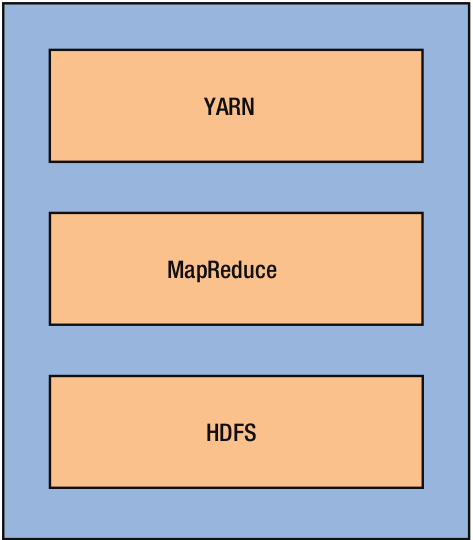
\includegraphics[width=0.4\textwidth]{hadoopCompo.png}
\caption{componenti principali di Hadooop}
\label{fig:hadoopComponets}
\end{figure} 
 
Uno dei fattori di successo di Hadoop è il basso costo. Hadoop è un sistema open-source che può essere eseguito su un cluster di commodity\footnote{hardware non dedicato di basso costo} hardware. Riesce cioè a garantire facilmente una scalabilità orizzontale aggiungendo al cluster, dei server poco costosi. Inoltre, riesce a garantire, via software la tolleranza ai guasti: assume che prima o poi vi saranno dei guasti e li gestisce in maniera trasparente. Uno sviluppatore software non dovrà preoccuparsi di gestire questi fault. Consente, cioè, di sviluppare applicazioni distribuite in maniera molto più semplice poiché viene sperata la logica di elaborazione dei dati dalla logica di distribuzione dei dati.
Hadoop è composto da tre componenti principali: un cluster mananger (YARN), un modello di computazione distribuito (Map-reduce) e un file system distribuito (HDFS)



 
 \subsubsection{Map Reduce}
 MapReduce \cite{Dean:2004:MSD:1251254.1251264} è il modello di computazione distribuita fornito da Hadoop. Mentre HDFS fornisce un file system distribuito per memorizzare grandi dataset, MapReduce fornisce un framework di computazione che consente di processare grandi dataset in parallelo attraverso un cluster di computer (nodi). Questo modello astrae la computazione distribuita fornendo dei costrutti ad alto livello che consentono di sviluppare facilmente applicazioni distribuite.
 Il framework MapReduce schedula in maniera automatica l'esecuzione di un applicazione su un insieme di macchine in un cluster, prendendosi carico  della gestione della comunicazione fra nodi, del bilanciamento del carico di esecuzione fra i nodi e dei possibili guasti dei nodi.
In questo modo, gli sviluppatori possono concentrarsi sulla logica di processing dei dati tralasciando questi dettagli.



 

Come suggerisce il nome stesso, questo modello si basa su due funzioni : \emph{map} e
\emph{reduce}. Tutti i carichi di lavoro in un applicazione MapReduce sono espressi implementando queste due funzioni. 


Tutti i carichi di lavoro in un applicazione MapReduce sono espressi implementando queste due funzioni.  
La funzione \emph{map} riceve in input una coppia chiave-valore e restituisce a sua volta una insieme di  coppie chiave valore intermedie. Il framework MapReduce esegue la funzione map per ogni coppia chiave valore presente nel dataset di input. L'output delle funzioni Map, è ordinato e raggruppato in base ai valori di chiave intermedi, e costituirà l'input della funzione Reduce. La funzione \emph{Reduce} aggrega i risultati della funzione map, in base al valore di chiave intermedio.
Fra la fase \emph{map} e la fase \emph{reduce}, vi è una fase intermedia detta \emph{shuffle} che consiste nel partizionare i dati in base al loro valore di chiave e indirizzarli al nodo reducer, ovvero il nodo su cui si dovrà eseguire la funzione \emph{reduce}.

I dati possono essere sia semi strutturati o non strutturati affatto, non è richiesto che i dati siano conformi ad uno schema rigido predefinito. L'unico requisito è che sia possibile esprimere il dataset in input come una serie di coppie chiave valore.
Il modello MapReduce ha rivoluzionato il modo di processare grandi datasets, offrendo un modello semplice che consente di scrivere programmi che possono essere eseguiti in parallelo su molte macchine. Grazie a questo, Map-Reduce consente di ottenere una scalabilità orizzontale: all'aumentare della dimensione dei dati è possibile aggiungere nuove macchine mantenendo quasi invariato il tempo di esecuzione.
\subsection{Apache Spark}
%Uno dei punti di forza del paradigma MapReduce, come abbiamo visto,  è quello di consentire all utente    di effettuare elaborazioni su larga scala senza che quest'ultimo di debba preoccupare di come distribuire la computazione sui vari nodi o come gestire i fallimenti di un nodo. Uno dei principiali svantaggi però di questo paradigma è dato dal fatto che non consente di implementare algoritmi che devono eseguire più iterazioni sugli stessi dati in maniera efficiente.
%Questa inefficienza è dovuta al fatto che i risultati intermedi della computazione vengono serializzati su filesystem.






Apache Spark \footnote{http://spark.apache.org/} è una framework open-source che consente di processare grandi dataset in maniera distribuita.
Spark può essere considerato come il successore del modello MapReduce di Hadoop, entrambi i framwork sono progettati per poter processare i big data.  Spark mantiene inalterata la scalabilità di MapReduce e la tolleranza ai guasti, e inoltre aggiunge nuove caratteristiche, offrendo inoltre ulteriori vantaggi rispetto a MapReduce. Primo fra questi è la velocità: Spark riesce a processare i dati riducendo  di molto i tempi di latenza (fino a 100 volte), poiché  consente ai nodi di processing di immagazzinare in memoria centrale i risultati intermedi, a differenza di MapReduce, dove invece erano serializzati sul file system.  



La velocità può essere talvolta un fattore determinante. Impiegare troppo tempo per processare i dati, rallenta tutto il processo decisionale riducendo il valore stesso dei dati.
La principale astrazione fornita da SPARK sono i \textbf{R}esilent \textbf{D}istributed \textbf{D}ataset (RDD) \cite{Zaharia:2012:RDD:2228298.2228301}, che essenzialmente sono una collezione immutabile e distribuita di oggetti. Questi oggetti sono, suddivisi in più partizioni che  generalmente sono distribuite su più nodi.

Questa astrazione permette agli sviluppatori di materializzare i risultati intermedi della computazione nella memoria dei vari nodi di processing. Ciò significa che i prossimi step che vogliono riconsultare questi dati, non li dovranno rielaborare o ricaricare da
disco. Per tale ragione, Spark  si presta bene per eseguire in parallelo sia algoritmi altamente iterativi che richiedono di scansionare un dataset di input
più volte, come gli algoritmi di machine-learning come   PageRank, K-means clustering, e logistic regression.




Architetturalmente, Spark è progettato per essere altamente accessibile: offre API per Python, Java, Scala, SQL e R. Inoltre si integra alla perfezione con strumenti di Big Data quali Hadoop (e strumenti che dipendono da esso come HBase, Hive, etc.) e Cassandra.




 
\begin{figure}[htbp]
    \makebox[\textwidth]{
        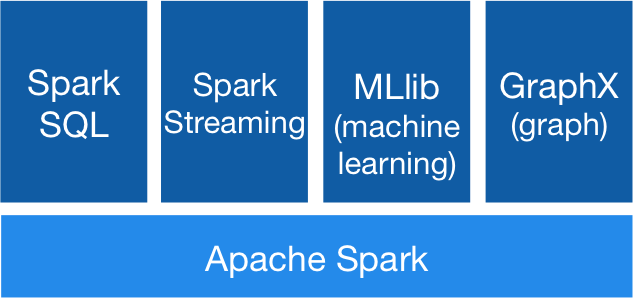
\includegraphics[width=0.7\textwidth]{spark-stack.png}
    }
    \caption{Stack applicativo Apache Spark}
    \label{fig:sparkstack}
\end{figure}




La figura \ref{fig:sparkstack} mostra le principali componenti di Apache Spark:
\begin{itemize}
\item \textbf{Spark Core}: contiene le funzionalità base di Spark fra cui l'astrazione sulla quale si basa l'intero ambiente, i \textit{resilient distributed dataset} (RDD).
\item \textbf{Spark SQL}: contiene le componenti per elaborare e manipolare dati strutturati. Permette l'interrogazione (tramite SQL) di dabatase relazionali, JSON, HIVE (mediante lo Hive Query Language) e file Parquet. 
\item \textbf{Spark Streaming}: componente che permette l'elaborazione di stream di dati.
\item \textbf{MLLib}: contiene algoritmi di Machine Learning per vari tipi di task quali classificazione, regressione, clustering, collaborative filtering, frequent pattern mining, dimensionality reduction, feature extraction e statistica di base.
\item \textbf{GraphX}: libreria per la manipolazione ed estrazione di conoscenza in grafi.
\end{itemize}

\subsection{Resilent Distribuited Dataset}
Formalmente un RDD è una collezione di oggetti immutabile e partizionata.
Questi RDD possono essere creati in due modi: o a partire da dati in un sistema di memorizzazione stabile\footnote{per stabile si intende fault-tolerant} (HDFS, Hive, Cassandra, ) o a partire da altri RDD, mediante un insieme di operatori messi a disposizione dal framework come map, reduce, groupByKey etc. 
Questo tipo di  operazioni, che creano RDD, sono dette \emph{trasformazioni}.
Un utente può controllare due aspetti fondamentali di un RDD: 
\begin{inlinelist}
  \item la loro persistenza,
  \item e può controllare il loro partizionamento
  
\end{inlinelist}
Se si ha intenzione di riutilizzare i dati in più step, l'utente può decidere di memorizzarlo nella cache dei nodi di processing, in modo tale che non venga  rielaborato. Inoltre è possibile che gli elementi di un RDD siano partizionati lungo le macchine nel cluster, in base al valore chiave di ciascun record.
Come vedremo in seguito questo meccanismo è molto utile per diminuire lo spostamento dei dati lungo la rete.

  Spark offre due tipologie di operazioni:
\begin{itemize}
\item \textbf{Trasformazioni} operazioni che producono nuovi RDD a partire da un rdd come \emph{map,filter,join}
\item \textbf{Azioni} queste operazioni invece restituiscono un valore al program-
ma Driver, dopo aver valutato una o più trasformazioni su un RDD.
\end{itemize}
A differenza di altri approcci di distribuzione dei dati che replicano i dati su più nodi, in spark per ogni RDD viene memorizzato il suo \emph{lineage} ovvero la sequenza di trasformazioni che lo ha prodotto, a partire da un altro RDD. In tal modo SPARK nel caso vi sia un failure, può rielaborare un RDD in maniera del tutto trasparente.
 
Gli RDD posssono contenere qualsiasi tipo di oggetti \footnote{poiche Spark è eseguito su una JVM, questi elementi sono oggetti JAVA} , che sono suddivisi in
partizioni in maniera automatica lungo il cluster. Questi oggetti una volta
creati, sono immutabili e possono essere creati solo tramite gli operatori
di Spark.
Ad esempio dato un RDD di coppie \texttt{(visitID,URL)} contenente le visiste di
alcuni siti internet, è possibile ottenere un nuovo RDD contenente per ciascun
sito il numero di visite ricevute \texttt{(URL,count)}, applicando l’operatore map
trasformando ogni coppia iniziale \texttt{(visitID,URL)} in una coppia \texttt{(URL,1)} e
poi applicando l'operatore \emph{reduce} per ottenere il numero di visite per ciascun sito.

In seguito è mostrato un frammento di codice in scala per ottenere tale
risultato:\\
\texttt{visits=spark.hadoopFile("hdfs://....")}\\
\texttt{val counts=visit.map(v=>(v.url,1)).reduceByKey( + )}\\

Una applicazione Spark consiste in un processo \textit{driver} e di un insieme di processi \textit{executors} distribuiti sui nodi del cluster (worker nodes) .
\begin{figure}[htbp]
    \makebox[\textwidth]{
        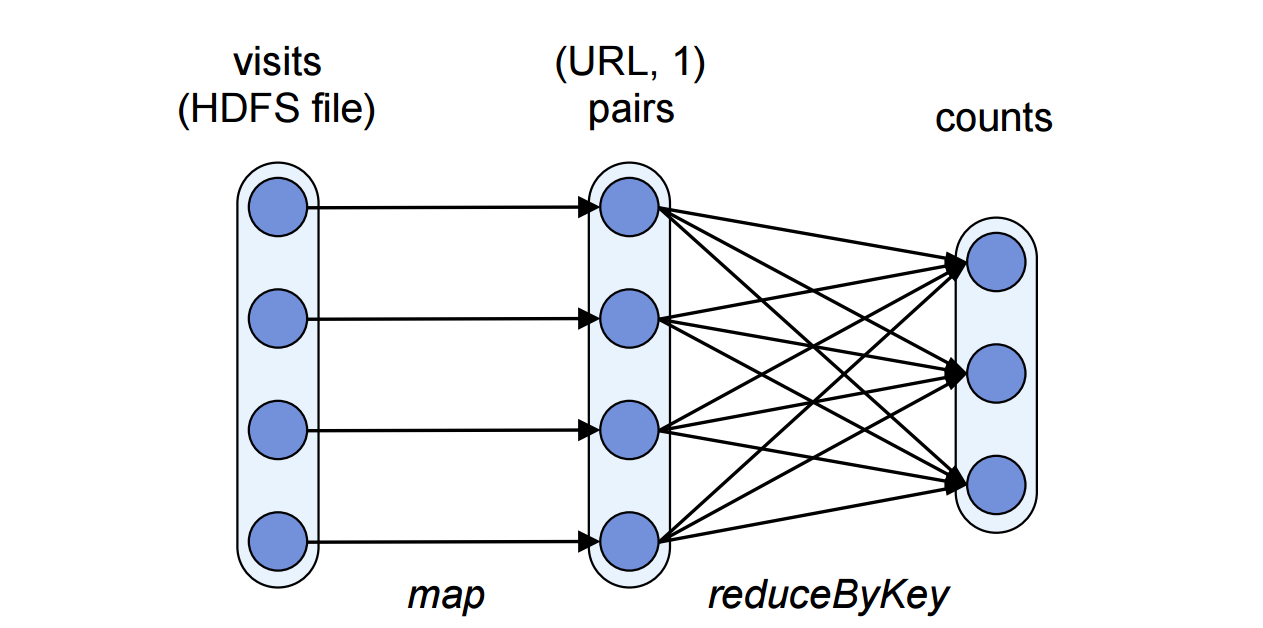
\includegraphics[width=0.7\textwidth]{sparkRDDexample.png}
    }
    \caption{Esempio di lineage Graph: Gli ovali rappresentano gli RDD, i pallini le partizioni}
    \label{fig:lineageRDD}
\end{figure}

La figura \ref{fig:lineageRDD} mostra il lineage-graph degli rdd in esempio. Se
viene persa una partizione dell'RDD \texttt{(URL,1)} sarà possibile ricalcolarla
rieseguendo l'operatore map, sulla corrispondente partizione.



Il processo (nodo)   driver dovrà gestire:
\begin{itemize}
\item interazione con l'utente;
\item coordinare e distribuire il flusso di controllo.
\end{itemize}


\begin{figure}[h]
\centering
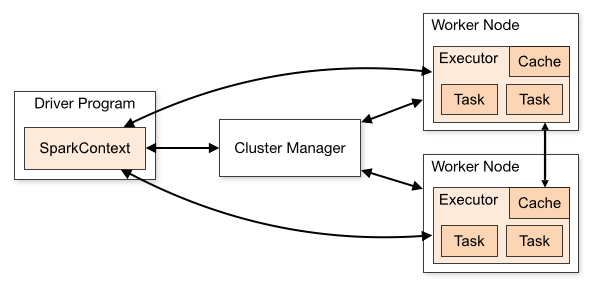
\includegraphics[width=0.8\textwidth]{cluster-ov.png}
\caption{componenti Di Un Cluster in Spark}
\label{fig:sparkClusterComponents}
\end{figure} 
 
I processi \lq\lq executor\rq\rq sono responsabili dell'esecuzione dei work in forma di \textit{tasks} e di memorizzare qualsiasi tipo di dato che l'utente sceglie di materializzare. 

In cima al modello di esecuzione vi sono i \textit{jobs}: l'invocazione di una azione all'interno di una applicazione Spark provoca l'esecuzione di uno Spark job in grado di soddisfare la richiesta. Spark esamina il grafo degli RDD dal quale l'zione dipende e produce un piano di esecuzione che inizia computando le risorse (gli RDD) in ordine di dipendenza, culminando con l'RDD che produrrà i risultati dell'azione.
 

Il piano di esecuzione consiste nell'assemblare trasformazioni di jobs in \textit{stages}. Uno stage corrisponde a una collezione di \textit{tasks} che eseguono simultaneamente lo stesso codice su una differenze partizione dei dati: ciascuno stage contiene una sequenza di trasformazioni che possono essere completati senza rimescolare i dati.

Quest'ultimo aspetto inficia fortemente le performance dell'applicazione. Una partizione di dati subisce un processo denominato "shuffling"  quando vengono effettuate trasformazioni \textit{narrow}, ad esempio una \textit{map}.

Il trasferimento dei dati fra i nodi del cluster avviene mediante un meccanismo di serializzazione: dopo questo processo, i dati vengono memorizzati in una cache e trasferiti in rete per uno shuffling. Spark prevede due meccanismi di serializzazione: l'approccio classico (utilizzando le API Java disponibile a partire dall'interfaccia \textit{java.io.Serializable}) e mediante la libreria \textit{Kryo}. Quest'ultima prevede un formato molto più compatto in grado di svolgere le operazioni in maniera più rapida.


\section{DBpedia}
Wikipedia \footnote{https://en.wikipedia.org/} è divenuta una delle maggiori risorse di conoscenza disponibili nel web, ed è manutenuta da migliaia di utenti (collaboratori). Gli articoli Wikipedia sebbene composti prevalentemente da testo, contengono informazioni semi-strutturate come: template infobox , informazioni sulla categorizzazione dell'articolo, immagini, geo-coordinate e link sia verso altre pagine web sia verso altre pagine wikipedia.
Gli infobox sono tabelle di coppie attributo valore, che mostrano i dati più rilevanti di ciascuna pagina wikipedia. Il progetto DBpedia \cite{Bizer:2009:DCP:1640541.1640848} estrae dati strutturati da wikipedia tramite un extraction framweork open source e li unisce in una base di conoscenza multi dominio e multi lingua. Per ogni pagina presente in wikipedia, viene associato un \emph{Uniform Resource Identifier (URI)} in DBpedia per identificare un'entità o un concetto descritto dalla corrispondente pagina Wikipedia della versione inglese. Durante il processo di trasformazione, i dati semi-strutturati come i campi infobox,categorie, pagelinks sono convertiti in triple RDF e aggiunte alla base di conoscenza come proprietà dell'entità identificata dall URI.  Per rendere omogenea la descrizione delle informazioni, è stata sviluppata un ontologia e sono state definite le corrispondenze fra le proprietà presenti negli infobox e l'ontologia.
L'ontologia DBpedia consisite di 320 classi e descritte da 1650 proprietà. Le classi organizzate mediante una gerarchia sussuntiva dove \emph{owl:Thing} è la classe più generale. Poiché Il sistema di Wikipedia infobox si è evoluto in maniera decentrata, talvolta accade ad esempio che si usino diversi template per la stessa tipologia di entità (class) o si usino nomi diversi per descrive lo stesso attributo (es placeOfBirth o birthPlace). 
 L'allineamento tra i template infobox e l'ontologia a causa di queste eterogeneità presenti nella nomenclatura, non è quindi completamente automatico, ma si basa anche su mapping definiti manualmente, forniti dalla comunità di DBpedia. Ad esempio ‘date of birth’ and ‘birth
date’ sono entrambi mappati con la proprietà birthDate. 
 
 La base di conoscenza DBpedia è disponibile sul web sotto GNU Free Documentation, e può essere consultata mediante varie modalità :
\begin{itemize}
\item \textbf{Linked Data}: linked data è la metodologia di pubblicazione  dei dati RDF nel web, che utilizza gli URI http come identificativo delle risorse e il protocollo HTTP per ritrovare al descrizione rdf delle risorse. Quando si accedere ad un URI di una risorsa DBPedia mediante un semantic web agent si ottiene la descrizione rdf della risorsa mentre se si utilizza un semplice web-browser si otterrà una vista html della descrizione.
\item \textbf{Sparql Endpoint } \'E fornito un endopoint mediante il quale si può interrogare la base di conoscenza tramite il protocollo SPARQL.
\item \textbf{RDF dumps} la base di conoscenza è stata suddivisa in varie parti in base agli rdf-predicate 
\end{itemize}
\chapter{Unsupervised Learning}
\label{cap:capitolo2}
% !TEX encoding = UTF-8
% !TEX TS-program = pdflatex
% !TEX root = ../tesi.tex
% !TEX spellcheck = it-IT

\section{DBSCAN}
L'algoritmo DBSCAN\cite{Ester96adensity} si basa sull'idea che ciascun elemento di un cluster debba avere un vicinato entro un certo raggio $\epsilon$ (anche chiamato $Eps$)  che contenga almeno un numero minimo di punti (MinPts). Questo algoritmo, in altre parole, stima la \emph{densità} di ciascun punto, per mezzo della cardinalità del suo vicinato entro un raggio predefinito $Eps$. 

A tal fine DBSCAN etichetta ogni punto in una delle sequenti categorie:\textit{ core-object, border-object} e \textit{noise}.
Un punto sarà definito come \emph{core-object} se la densità del suo eps-vicinato supera la soglia $MinPts$.
A partire da questi punti core vengono definite delle proprietà di connettività verso  tutti quei punti che appartengono al eps-vicinato.


In seguito verranno date le definizioni formali delle proprietà di connettività fra i punti, che verranno utilizzate per generare i possibili cluster.
 %defizioni di DBSCAN
\begin{definizione}[directly density-reachable]
\label{def:ddr}
Un oggetto $p$ si dice 	\emph{directly-density-reachable} da un oggetto $q$ rispetto ai parametri $Eps$ ed $MinPts$ nell'insieme di oggetti $D$ se:
\begin{enumerate}
\item $p \in Neigh_{eps(Q)}$
\item $|Neigh_{eps(Q)}| \ge MinPts$
\end{enumerate}
\end{definizione}
\begin{definizione}[density-reachable]
\label{def:dr} 
Un oggetto   $p$ si dice 	\emph{"density-reachable"} da un oggetto $q$ rispetto ai parametri $Eps$ ed $MinPts$ nell'insieme di oggetti $D$, e si  indica con \emph{$p>_{D}q$}, se esiste una catena di oggetti: $p_1,\dots,p_n$, $p_1=p\; p_n=q$ tali che:  $p_{i} \in D  \land p_{i+1}$ è \emph{directly density-reachable} da $p_{i}$
\end{definizione}
Questa relazione è l'estensione canonica della relazione di  Directly density reachability. Ovvero se abbiamo che un punto $p$ è ddr\footnote{ddr=directly density reachable} a q, e q è ddr da $r$ allora diremo che $p$ è \emph{density reachable} da $r$.
Inoltre è una relazione transitiva ma non simmetrica. Sebbene non sia simmetrica, vi sono delle zone nell'isnieme $D$, in cui questa relazione è simmetrica ovvero  per quegli oggetti $o$ nell insieme per cui $|N_{eps(o)}| \ge MinPts$. Due oggetti \emph{border}, ovvero due oggetti che giacciono sul confine di un cluser, probabilmente non saranno density-reachable fra loro in quanto non ci sono abbastanza oggetti nel loro vicinato. Tuttavia, ci sarà necessariamente, un terzo oggetto nel cluster dal quale entrambi questi  oggetti border saranno density-reachable.
%figura esempio
\begin{figure}
\centering
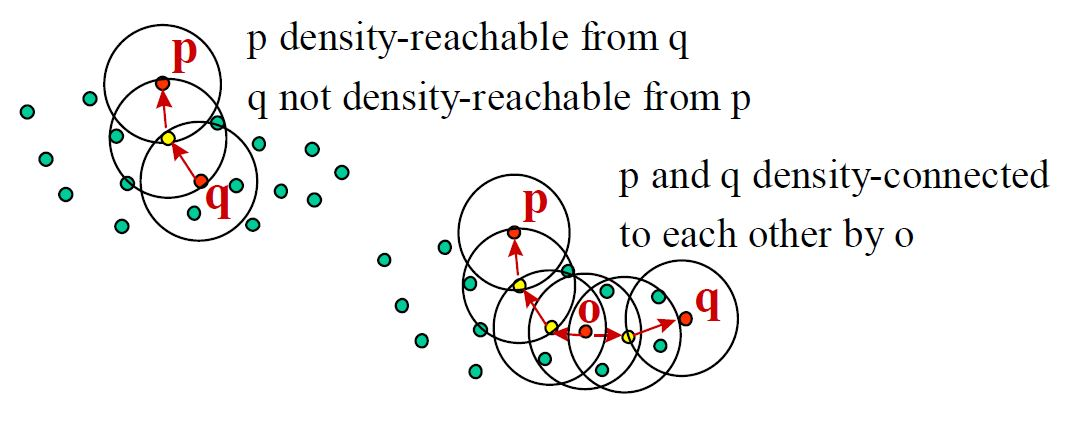
\includegraphics[width=0.6\textwidth]{density-reachable}
\caption{Density Reachability e Density Connectivity}
\label{fig:dens-reach}
\end{figure}
%density connected def
\begin{definizione}[density-connected]
\label{def:dc}
Un oggetto $p$ si dice 	\emph{"density-connected"} da un oggetto $q$ wrt $Eps$ ed $MinPts$ nell'insieme di oggetti $D$ se esiste un oggetto $o \in D$  tale che sia $p$ che $q$ siano \emph{ density reachable} da $o$. La relazione di density-connectivity è simmetrica, la figura \ref{fig:dens-reach} mostra la le definizioni su descritte in uno spazio bi-dimensionale. 
\end{definizione} 
Proprio grazie alla proprietà di density connectivity, si potrà dare la definizione di cluster ovvero un insieme massimale di oggetti \lq\lq densamente connessi\rq\rq.
%cluster def
\begin{definizione}[cluster]
\label{def:cluster}
Sia $D$ un insieme di oggetti.
Si defnisce \emph{\lq\lq cluster\rq\rq}  $C$,  wrt $Eps$ ed $MinPts$ nell'insieme di oggetti $D$,
un sottoniseme non vuoto di $D$, che soddisfa le seguenti condizioni :
\begin{enumerate}
\item \emph{Massimalità}: $\forall p,q\in D$, se $p \in C \land q>_{D}p$ wrt MinPts e Eps, 
allora anche $q \in C  $

\item \emph{Connettività}: $\forall p,q\in C$, $p$ è \emph{"density-connected"} a $q$  wrt MinPts e Eps

\end{enumerate}
 
\end{definizione} 


%def noise
\begin{definizione}[noise]
\label{def:noise}
Siano $C_1,\dots,C_k$ tutti i cluster wrt Eps e , ovvero come un insieme di oggetti densamente connessi che è massimale rispetto MinPts in $D$. Si definisce \emph{noise}  l'insieme di oggetti $D$ che non appartengono a nessun cluster $C_i$,
noise=$\lbrace p\in D | \forall i: p \notin C_i \rbrace $.
 
\end{definizione}
Questo algoritmo presenta due proprietà fondamentali che ne permettono una computazione efficiente:
\begin{enumerate}
\item Dato un qualsiasi core-object, l'insieme dei punti density reachable da tale punto (w.r.t Eps,MinPts) costituirà un cluster.
\item  Si consideri un cluster $C$, ciacun elemento di C è density-reachable da  un ogni core-object in C. Ciascun cluster sarà quindi, univocamente identificato da uno qualsiasi dei suoi core-object.
\end{enumerate}

L'algoritmo di DBSCAN, al fine di creare un cluster,parte da un punto arbitrario $p$ e ritrova tutti i punti da esso density-reachable rispetto ai parametri $Eps$ e $MinPts$, effettuando region-query \footnote{una region-query  di un punto $p$ è la ricerca dei punti che ricadono nel viciniato di $p$} prima per $p$ ed eventualmente per i vicini di p diretti ed indiretti.
Se l'oggetto $p$ è un core-object tale procura ci darà un cluster, altrimenti l'oggetto $p$ sarà considerato come NOISE, e si passerà al oggetto successivo. Se $p$ è un border-point sarà successivamente ri-etichettato quando, verrà considerato un core object dal quale $p$ è density reachable.
Le implementazioni classiche di DBSCAN fanno uso di indici spaziali come R-tree o X-tree, che consentono di ritrovare il viciniato di ciacun punto (region-query) in maniera efficiente $O(logn)$. Nel peggiore dei casi, DBSCAN visita ogni punto del dataset, ovvero esegue una region query per ciascun punto, ciò determina una complessità $0(n^2)$  dove $n$ rappresenta il numero di punti nel dataset. Se si utilizza una struttura indicizzata come un R-tree, è possibile passare ad una coplessità $0(nlogn)$ . 
Tali strutture indicizzate però, non riescono a scalare all'aumentare della dimensionalità dei dati: la performance delle region query passa da  O(logn)to O(n), facendo degenerare, cioè la complessità temporale di dbscan in $O(n^2)$ rendendo poco adatto questo algoritmo al problema del clustering dei tweets. Nel lavoro di Guo et al. \cite{4370588} vien proposto una variante dell'algoritmo DBSCAN che fa uso dell'LSH, al fine di ritrovare i nearest-neighbors di un punto, riducendo sensibilmente la complessità dell'algoritmo.
 
 %note dbscan
L'algoritmo DBSCAN riesce  a generare dei cluster anche con un elevata presenza di rumore. Inoltre grazie alla definizione di "density-connected"\ref{def:dc}, riesce ad identificare cluster di forme arbitrarie. Inoltre, a differenza di altri algoritmi come k-means, non necessita di conoscere a priori il numero di cluster. Tutte queste caratteristiche rendono questo algoritmo particolarmente interessante nella scoperta di cluster in questo lavoro di tesi poiché: i messaggi di un microblog come Twitter contengono un'alta percentuale di rumore, e nel task di event-detection non è possibile sapere a priori il numero di eventi.
\subsection{DBSCAN come ricerca di componenti connesse }
Il problema del clustering, può essere ricondotto al problema della ricerca di componenti connesse in un grafo.
In un grafo, una \emph{componente connessa} è un sotto-grafo in cui ogni coppia di vertici è connessa da un cammino, e il sottografo non è connesso  a nessun altro vertice  del grafo di partenza. Per ottenere una corrispondenza fra una  componente ed  un cluster secondo dbscan, sarà sufficiente far sì che per ogni coppia di punti  density-connected, esista un cammino che li colleghi.
\begin{figure}
    \centering
    \begin{subfigure}[b]{0.45\textwidth}
        \centering
        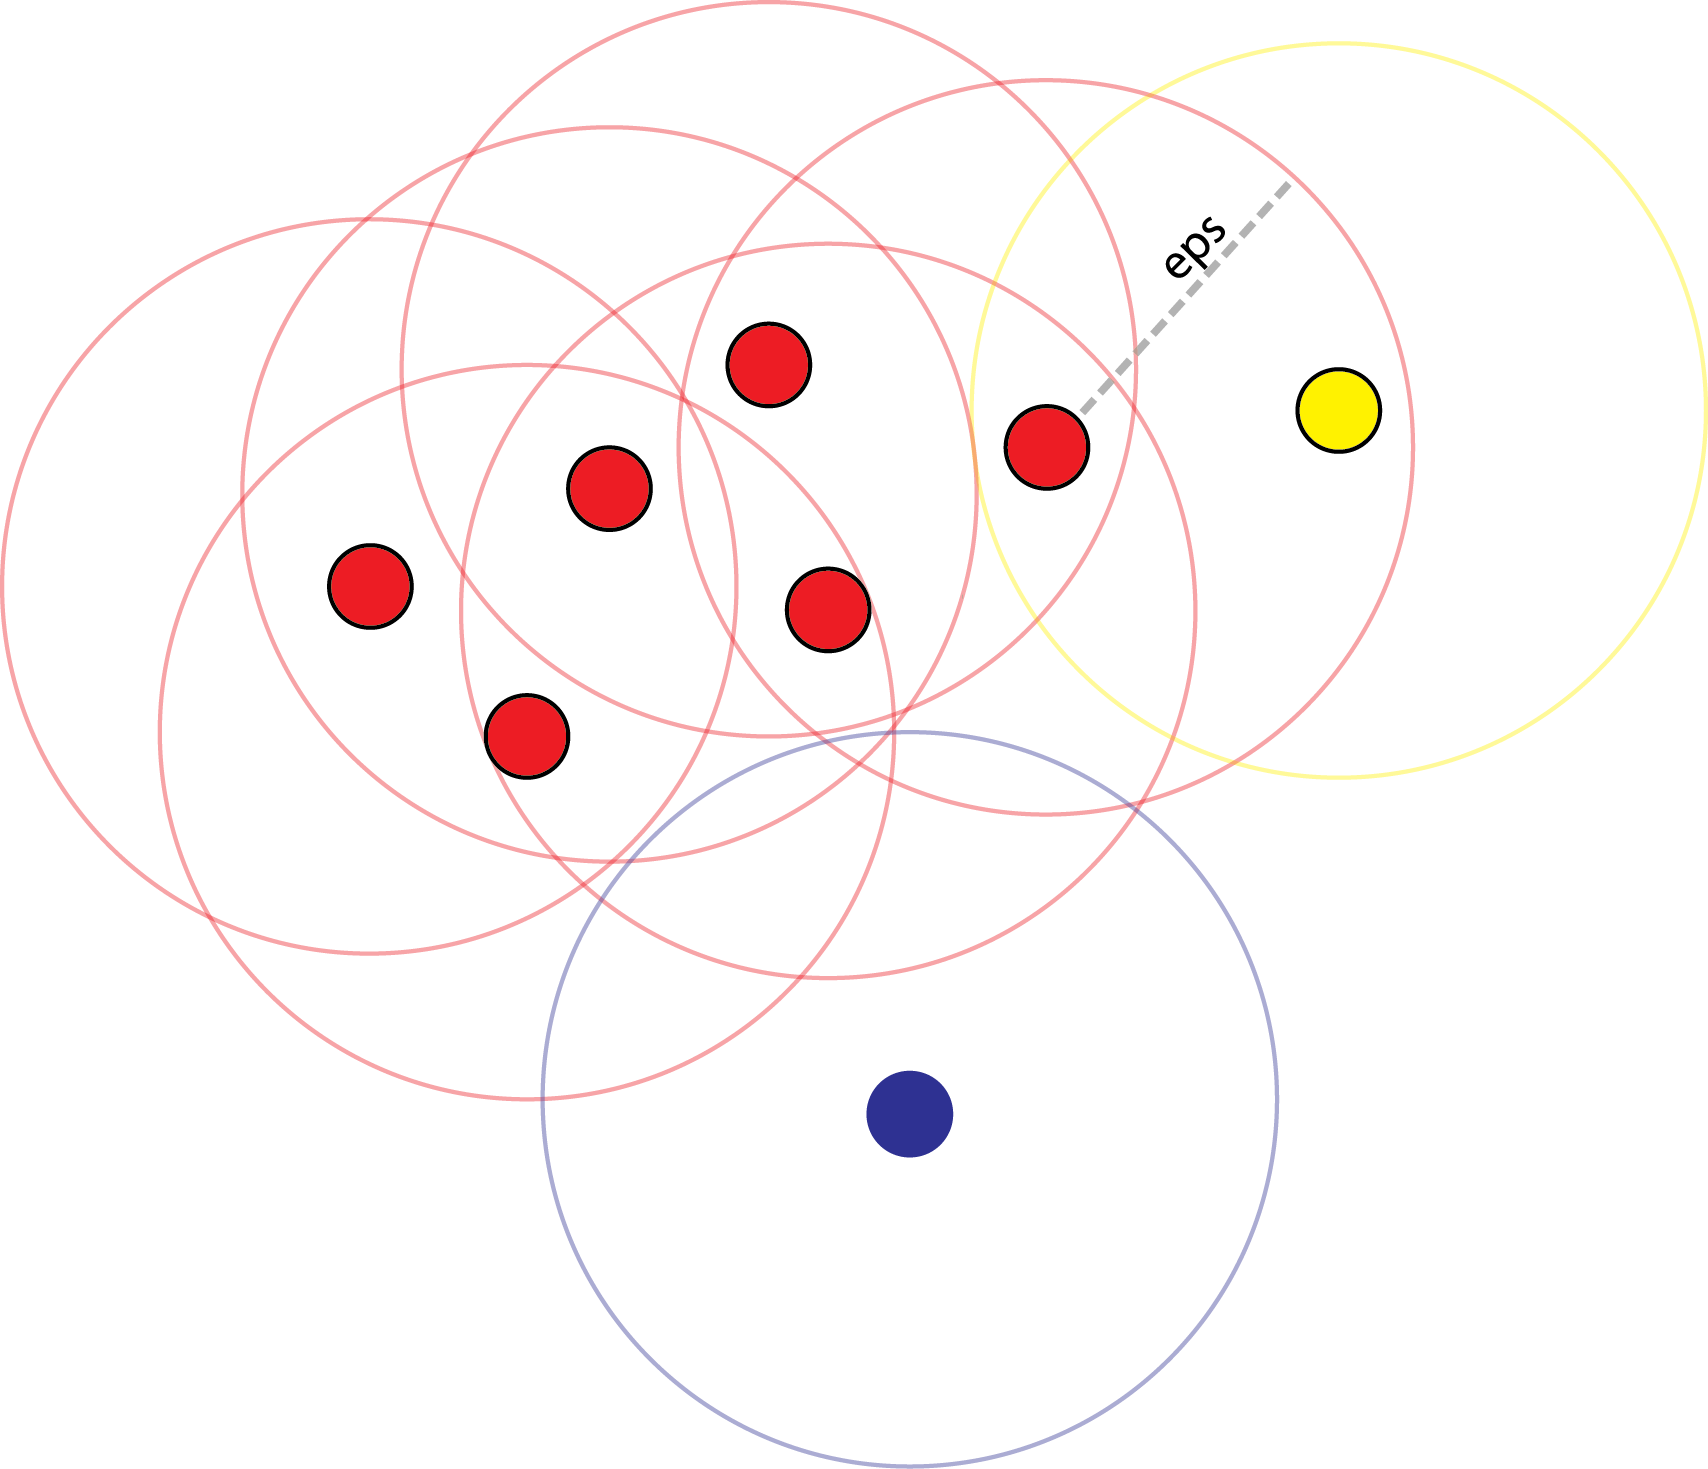
\includegraphics[width=\textwidth]{dbscanWithoutPaths}
       	\caption{ MinPts=3}
         \label{fig:densityConnectedObjects}
    \end{subfigure}
    \hfill
    \begin{subfigure}[b]{0.45\textwidth}
        \centering
        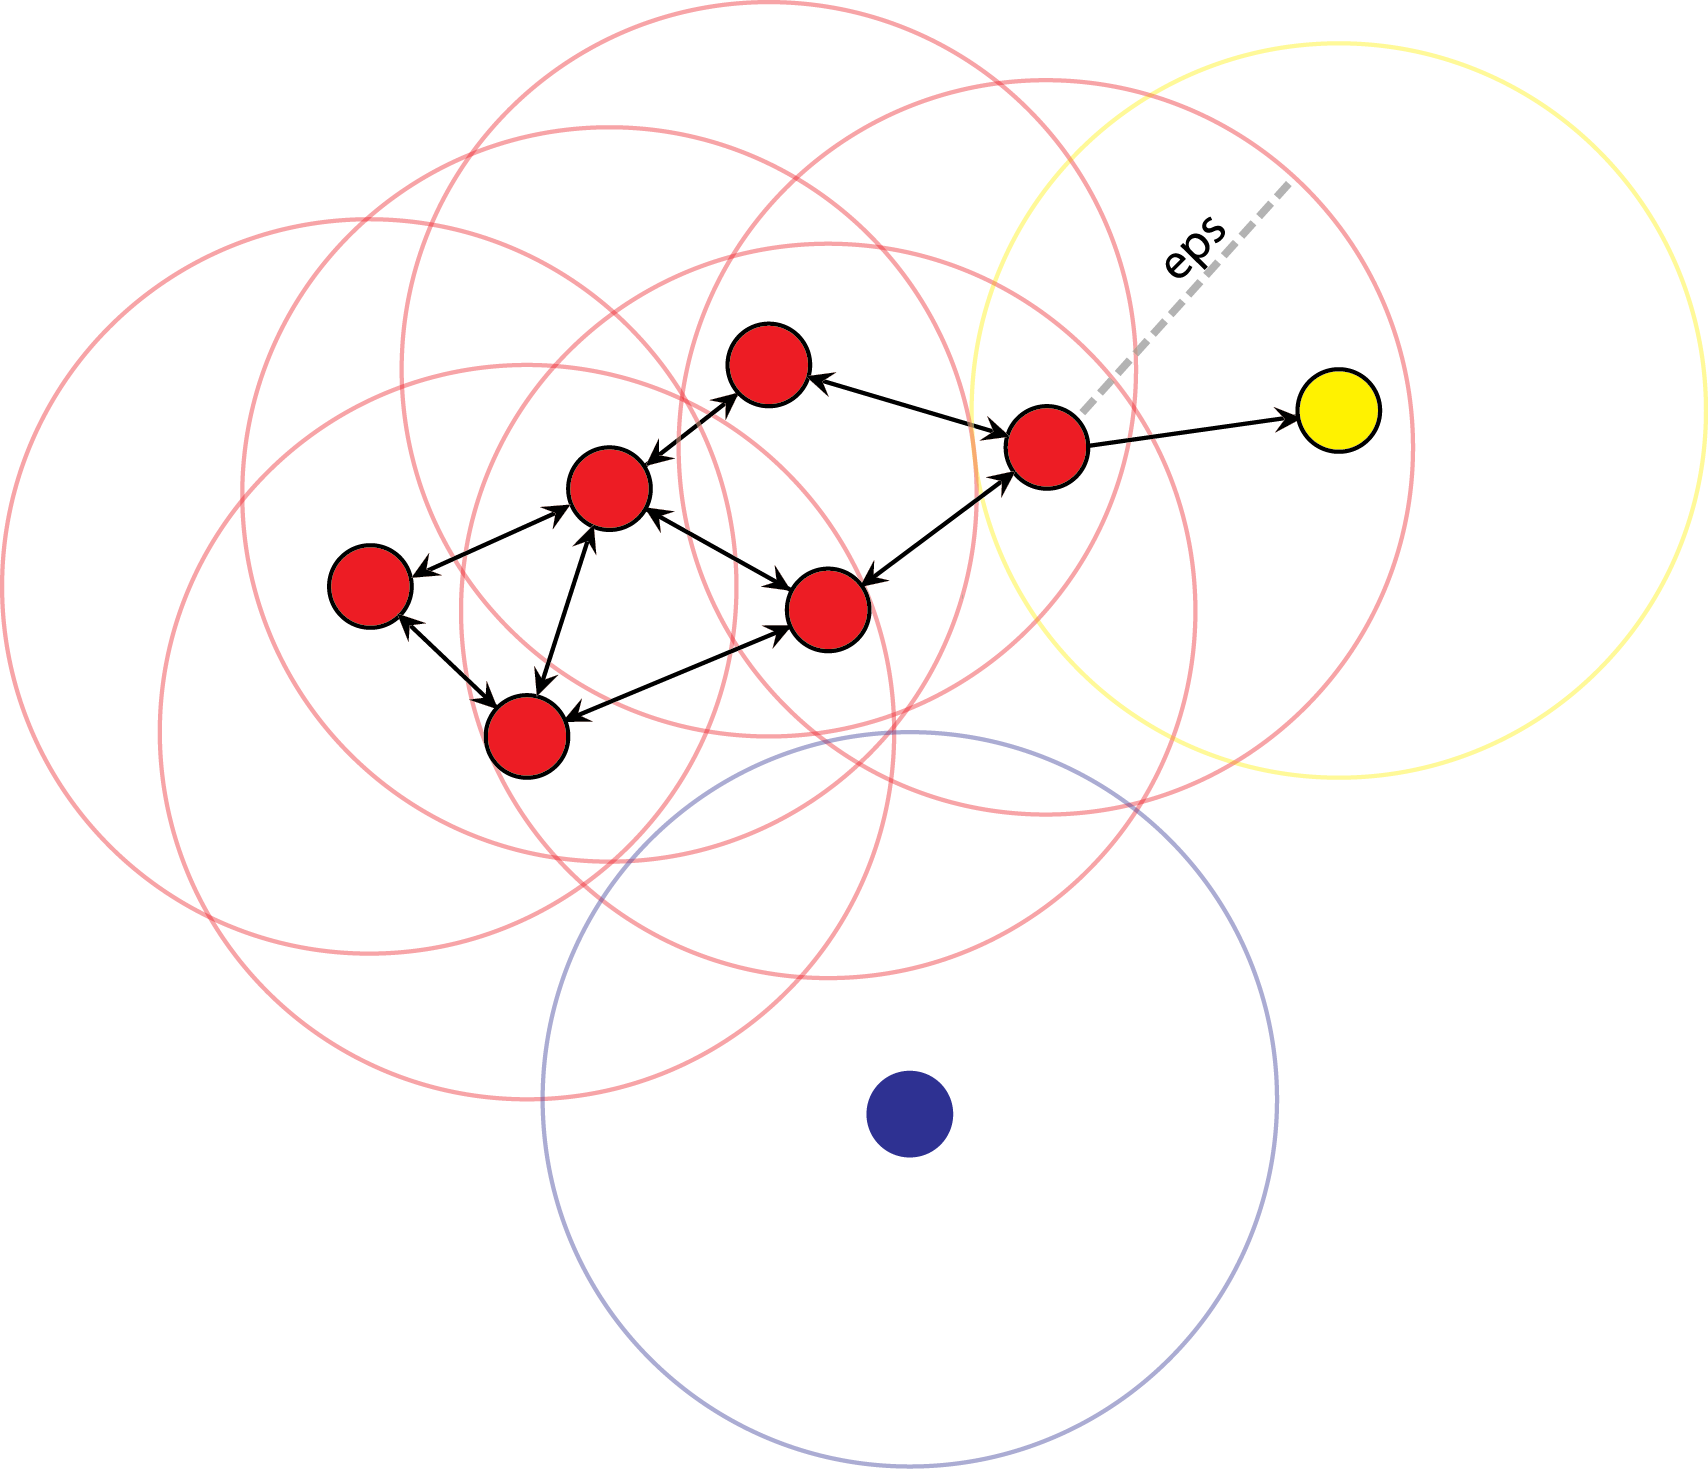
\includegraphics[width=\textwidth]{dbscanPaths}
        \caption{Esempio di grafo di densità}
         \label{fig:graphdensityConnectedObjects}
    \end{subfigure}
    \hfill
    \caption{rossi=core-objects, gialli=border,
    	blue=noise}
    \label{fig:dbscangraph}
\end{figure} 
In figura \ref{fig:graphdensityConnectedObjects} è mostrato come è possibile rappresentare un grafo non diretto a partire da connessioni di densità: per ogni coppia di oggetti di  directly density reachable $a,b$ con $a$ core-object,
verrà creato un arco $(a,b)$.
Talvolta però, un border-object può essere nel vicinato di più di un core-object anche appartenenti a cluster distinti, come mostrato in figura \ref{fig:dbscanGraphRevisited}. Se fossero lasciati entrambi gli archi verso il border-object, verrebbe identificata un'unica componente connessa. Lasciare questi archi renderebbe l'algoritmo molto più sensibile al rumore, poiché  un solo punto (magari un noise) potrebbe determinare la fusione di più cluster.

Per evitare tali problematiche, bisogna costruire un grafo i cui nodi sono sono soltanto i \emph{core-objects}, e verrà aggiunto un arco fra due nodi solo se la loro distanza è minore di $eps$.  In maniera più formale il grafo è cosi definito:

$
G=(V,A) \:$ dove :

$ V= \lbrace x \in D \:| \: Card(Neigh_{eps(x)}) \ge MinPts\rbrace$


$ A= \lbrace (x,y) \in V \:| \: d(x,y) \le eps \rbrace$

A partire da questo grafo $G$ verranno identificate tutte le componenti connesse che corrispondo ai cluster, individiuati però solo a partire dai nodi cores. Bisognerà quindi eseguire un ulteriore step per assegnare gli oggetti border ad un cluster con cui sono connessi. L'algoritmo originale nel caso in cui un oggetto border   ricada nel vicinato di più core objects, ciascuno dei quali di un cluster differente, lo assegnerebbe in maniera  casuale ad uno di questi cluster. In questo caso è possibile adottare tre strategie diverse:
\begin{itemize}
\item scegliere in maniera casuale un cluster 
\item scegliere il cluster con cui il border object ha maggiore connettività 
\item scegliere il cluster più vicino al border object
\end{itemize}

\begin{figure}
\centering
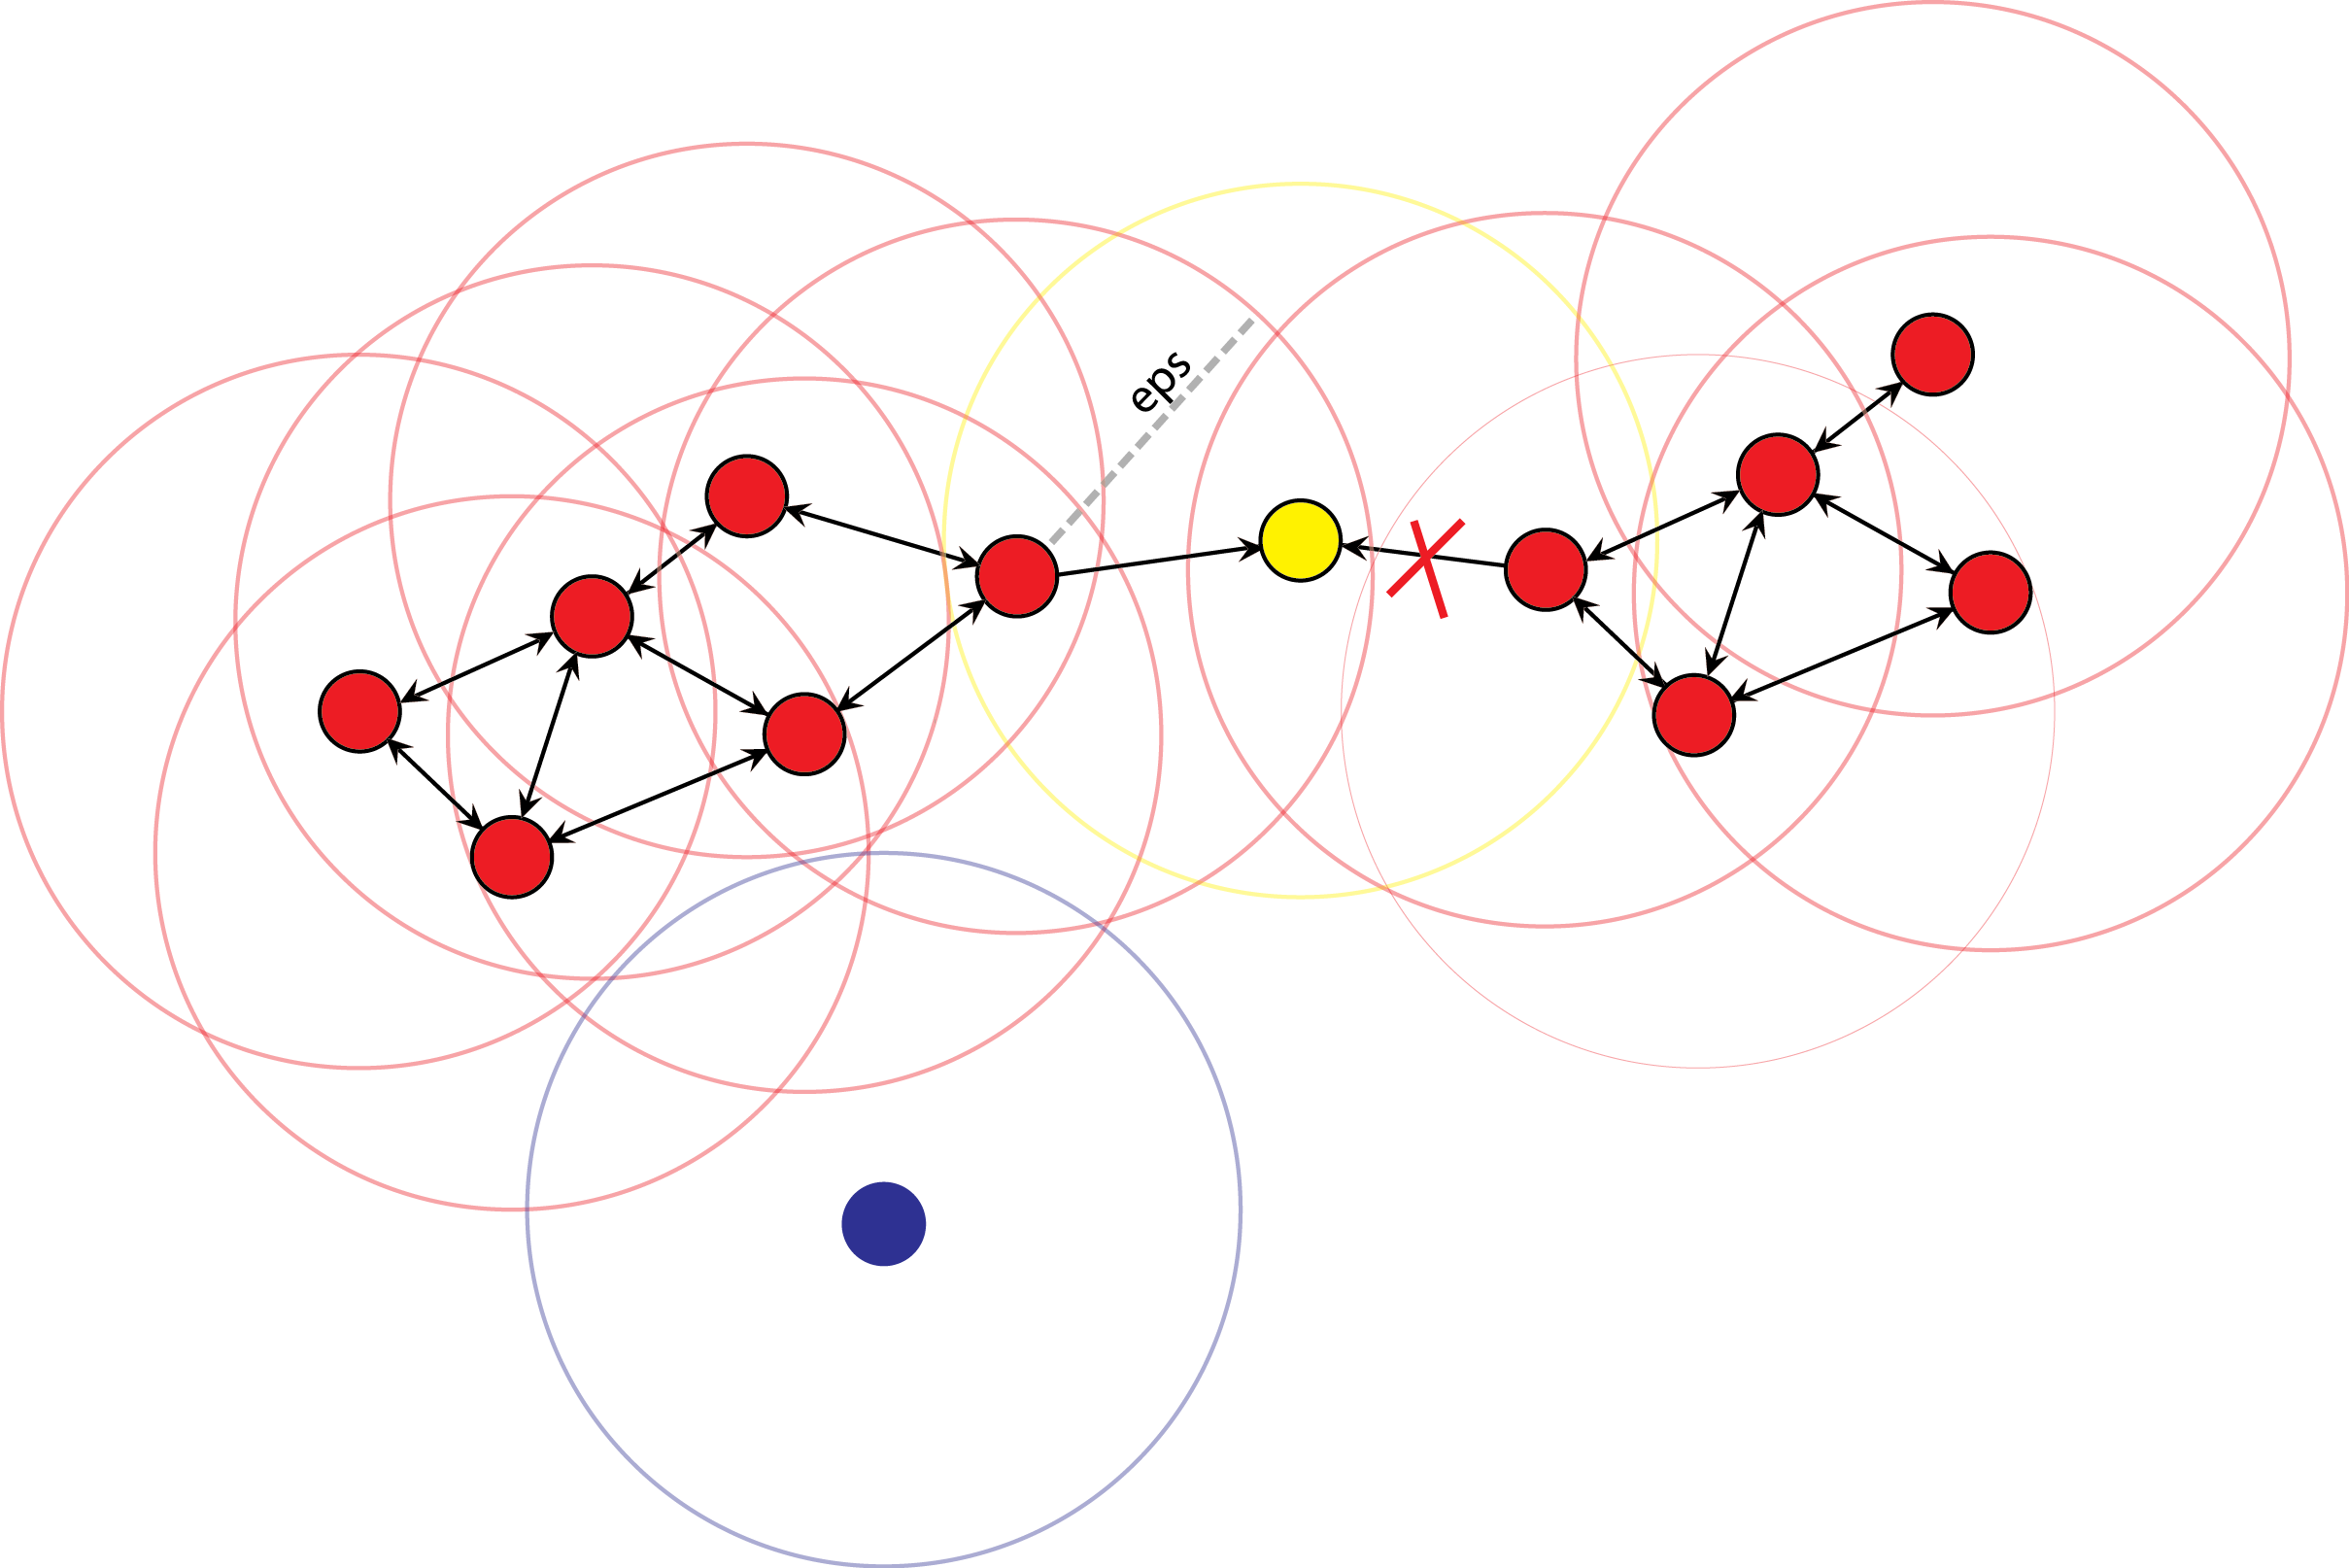
\includegraphics[width=0.6\textwidth]{dbscanRevisited}
\caption{border object density reachable da due core-object}
\label{fig:dbscanGraphRevisited}
 \end{figure}
%density connected def
 
 


\section{Sensitive Hashing}
Un problema fondamentale che molti task di Data Mining devono affrontare è quello di esaminare i dati per trovare item "simili". Molto spesso questo problema è risolto cercando il Nearest Neighbor ( o i primi k-nearest neighbor) di un oggetto in qualche spazio metrico $R^d$ .
Nel caso di poche dimensioni (d=2, d=3) questo problema, si riesce a risolvere in maniera piuttosto efficiente (O(log n)) mediante l'utlizzo di strutture dati come K-D-Tree o R-tree che partizionano lo spazio delle feature. Tuttavia al crescere delle dimensioni (curse of dimensionality), queste strutture basate sul partizionamento dello spazio, degradano in una ricerca lineare \cite{Weber:1998:QAP:645924.671192} passando quindi ad una complessità quadratica.
Per rendere meglio l'idea supponiamo di voler calcolare i documenti più simili in una collezione composta da un milione di documenti, si avrebbero quindi  $\binom{100000}{2}$  coppie di cui calcolare la similarità. Se ci si impiega un microsecondo per ogni calcolo di similarità, sarebbero necessari quasi sei giorni per valutare tutte queste coppie.
Se l'obiettivo è proprio il calcolo delle similarità di ogni possibile coppia, l'unico modo per ridurre il tempo necessario è usare una qualche forma di parallelismo. Tuttavia spesso, come nel caso del NNS-problem, si è interessati solo alle coppie più simili o più in generale a quelle coppie la cui similarità è al di sopra di una determinata soglia. \'E quindi sufficiente considerare solo quelle coppie che "probabilmente" sono simili, piuttosto che considerarle tutte. Proprio a tale scopo, se la dimensionalità dei dati è piuttosto alta, è possibile usare la tecnica del \emph{Local Sensitive Hashing} (LSH) \cite{Lsh} \cite{Gionis:1999}. L'idea chiave dell'LSH è quella di eseguire l'hasing dei punti attraverso molte funzioni di hashing, in modo tale che per ogni funzione la probabilità di collisione sia più alta per i punti vicini fra loro, rispetto ai punti più distanti.
Dopo aver eseguito l'hashing  tutte le coppie che sono state mappate nello stesso "bucket" possono essere considerate come \emph{coppie candidate}, solo queste coppie saranno valutate per determinare quali sono realmente simili. Quello che ci si augura è che, le coppie di item fra loro dissimili non vegano mai mappate verso lo stesso bucket,tali coppie rappresentano infatti dei \emph{false positive}. Allo stesso tempo ci si auspica che tutte (o la maggior parte) delle coppie realmente simili siano mappate nel medesimo bucket, le coppie che simili che non sono ricadute nello stesso bucket rappresentano i \emph{false-negative}
\subsection{Teoria dell'LSH}
 L'LSH è un framework per costruire strutture dati che permettono di ricercare i "near neighbor" all'interno di una collezione di vettori altamente dimensionali.  Dato un insieme $P$ contenente vettori D-dimensionali, l'obiettivo è di costruire una struttura che consenta di ritrovare, per un qualsiasi query point $q$, tutti quei punti che giacciono in un raggio di distanza $cR$ (dove $c$ rappresenta un fattore di approssimazione $>1$), o più formalmente gli \emph{R-near neighbors} di q.
 Data una funzione di hashing $h$ diremo che una coppia di oggetti $(x,y)$ sarà una \emph{candidate}   se $h(x)=h(y)$. Sia $d(\cdot,\cdot)$ una qualche funzione  definita su un insieme di oggetti $S$
\begin{definizione}[Locality-sensitive hashing] 

Una famiglia di funzioni $H$ si dice $(d_1,d_2,p_1,p_2)-Sensitive$ se  $\forall (x,y) \in S ,\;\forall h \in H $ 


\begin{itemize}
\item $se \quad  d(x,y)\leq d_1 \Rightarrow P_H[h(x)==h(y)]\geq p_1  $,
\item $se \quad  d(x,y)\geq d_2 \Rightarrow P_H[h(x)==h(y)]\leq p_2  $
\end{itemize}
dove $p_1>p_2$
\end{definizione}
A differenza di algoritmi di hashing classici dove si cercano di evitare delle collsioni per item diversi, in questo caso si cerca di massimizzare la probabilità di collisione per item vicini.
Dato un oggetto $q$ come query, verranno restituiti gli oggetti che giacciono nello stesso bucket $h(q)$
 

\begin{figure}[h]
\centering
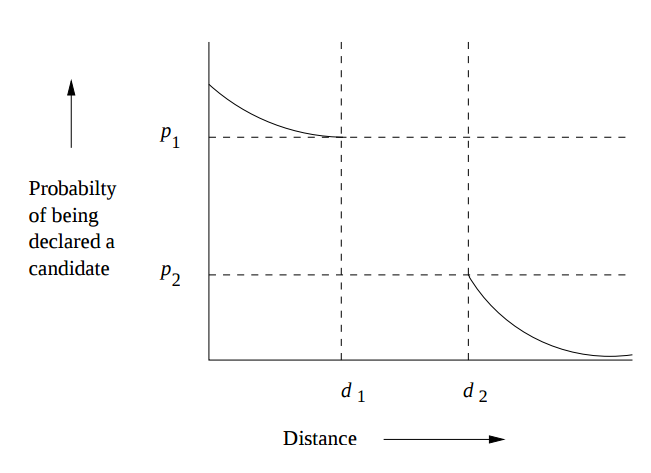
\includegraphics[width=0.6\textwidth]{hashFamily.png}
\caption{esempio di una funzione $(d_1,d_2,p_1,p_2)-sensisitve$}
\label{fig:lshfamily}
\end{figure} 
 
La figura \ref{fig:lshfamily} mostra un la probabilità che una possibile funzione di una famiglia  $(d_1,d_2,p_1,p_2)-sensisitve$ dichiari una coppia come candidata.

Data una famiglia di funzioni hash $(d_1,d_2,p_1,p_2)-sensisitve$ \emph{H} si può costruire una nuova famiglia di funzioni \emph{H'} applicando la \emph{AND-construction} su H come segue: ciascuna funzione di H' sarà data dalla concatenazione  da $r$ funzioni di H : $\lbrace h_1....h_r \rbrace $. Allora per ogni funzione $h$ in \emph{H'} diremo che: $h(x)=h(y)$ se $h_i(x)=h_i(y)$ per ogni $i...r$.  Dato che le funzioni $h_i$ sono scelte in maniera indipendente da $H$, possiamo asserire che \emph{H'} è una famiglia $(d_1,d_2,p_1^r,p_2^r)-sensisitve$.
Se invece costruiamo una nuova famiglia di funzione, per mezzo di una disgiunzione di \emph{b} elementi  di \emph{H} (\emph{OR-construction}), passeremo da una famiglia  $(d_1,d_2,p_1,p_2)-sensisitve$ ad una  $(d_1,d_2,1-(1-p_1)^b,1-(1-p_2)^b)-sensisitve$ \emph{H'}. In questo caso diremo che: $h(x)=h(y)$ se esiste  un valore di $i$ tale che $h_i(x)=h_i(y)$ 
Se $p$ è la probabilità che elemento di \emph{H} dichiari una coppia $(x,y)$ come candidata, allora $1-p$ è la probabilità che non lo sia. Avendo $b$ funzioni $h_1,...,h_b$ avremo che la probabilità che nessuna di esse dichiari la coppia come candidata, pari a   $(1-p)^b$ , e di conseguenza $1-(1-p)^b$ sarà la probabilità che almeno una fra le $b$ funzioni dichiarerà la coppia come candidata.
\'E facile notare che la \emph{And-Construction} fa decrescere tutte le probabilità, mentre la \emph{OR-construction} ha l'effetto opposto.\'E però possibile, applicare in cascata queste due tecniche AND,OR in modo tale che la probabilità $p_2$ sia più bassa possibile, mentre $p_1$ sia quanto più possibile vicino ad 1, ottenendo a una famglia $(d_1,d_2,1-(1-p_1^r)^b,1-(1-p_2^r)^b)-sensisitve$. Scegliendo in maniera accurata i valori di $r$ e di $b$ sarà possibile controllare l'andamento della funzione di probabilità $1-(1-p^r)^b$.
Tale funzione, una volta fissati i parametri $r$ e $b$, descrive una \emph{S-curve}. Come per qualsiasi \emph{S-curve}, è possibile determinare il punto fisso, ovvero quel valore di $t$ che rimane inalterato dopo aver applicato, la funzione $p=1-(1-p^r)^b$. Tale valore può essere approssimato come $t\approx (1/b)^\frac{1}{r}$. Al di sotto di tale soglia, il valore di probabilità decresce,al di sopra cresce.Quindi, se  se scegliamo la probabilità più alta $p_1$ al di sopra della soglia $t$, e $p_2$ al di sotto, avremo che il valore  $p_2$ è ridotto e al contempo il valore $p_1$ viene innalzato. Bisogna quindi impostare i valori di $b,r$ in modo tale che il punto fisso della funzione, corrisponda proprio al valore di similarità tale per cui due elementi li possiamo considerare "simili".
\begin{figure}
    \centering
    \begin{subfigure}[b]{0.45\textwidth}
        \centering
        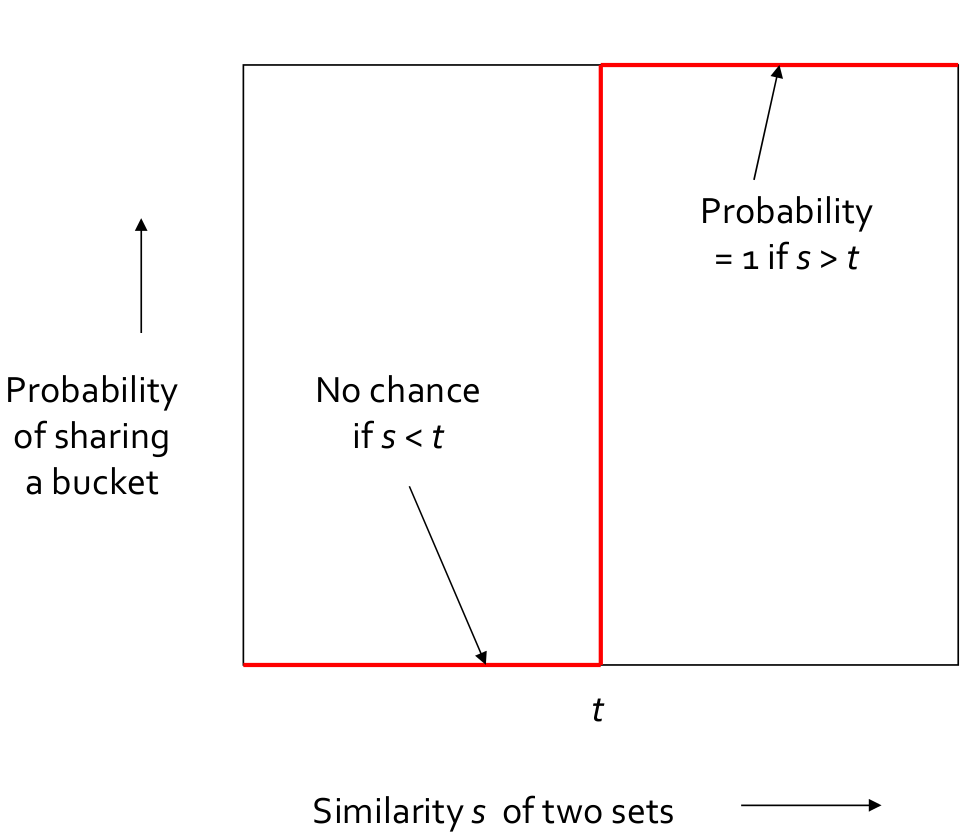
\includegraphics[width=\textwidth]{perfectSCURVE}
        \caption{s-curve ideale}
        \label{fig:perfectScurve}
    \end{subfigure}
    \hfill
    \begin{subfigure}[b]{0.45\textwidth}
        \centering
        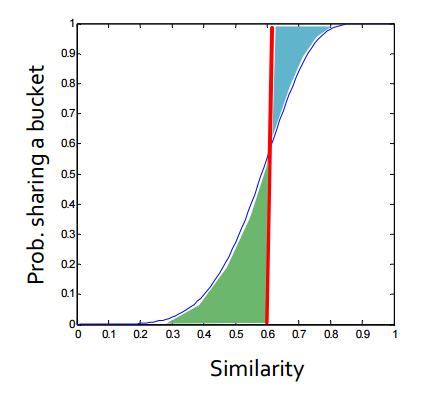
\includegraphics[width=\textwidth]{s-curve}
       \caption{s-curve r=5,b=10}
        \label{fig:realscurve}
    \end{subfigure}
    \hfill
    
    \caption{esempi di S-Curve}
    \label{fig:scurve}
\end{figure} 
La figura \ref{fig:perfectScurve}  mostra il caso ideale: dopo un valore di soglia la propabilità che due una coppia diventi candidata diviene immediatamente pari a 1, al di sotto pari a zero. Nella figura \ref{fig:realscurve} viene mostrato invece il caso in cui $r=5,b=10$, l'area verde indica il false-positive rate, mentre l'area blue indica il false negative rate.
Bisogna quindi, effettuare un tuning dei parametri $b,r$ per cercare di ritrovare la maggior parte delle coppie di elementi realmente simili, e al contempo avendo pochi false-positive.
Bisogna tenere a mente, però , che i false-positive possono essere filtrati con una fase di post-processing valutando la similarità reale fra le coppie restituite, i false negative, invece non possono essere in alcun modo recuperati, poiché rappresentano quelle coppie di item la cui distanza è bassa, ma che non sono state mappate nello stesso bucket.
\bibliographystyle{plain}
\subsection{LSH-Cosine}
In questo lavoro di tesi poiché si stanno analizzando documenti testuali, verrà utilizzata una famiglia di funzioni di hashing local-sensitive per la distanza del coseno. In particolare sarà adottato lo schema di lsh proposto da Charikar\cite{Charikar:2002:SET:509907.509965} in cui la   la probabilità che due punti collidano (ovvero che siano mappati verso lo stesso bucket), è proporzionale al coseno dell'angolo fra di loro. Data una collezione di vettori in $R^d$ viene definita una famiglia di funzioni hashing come segue: si sceglie un vettore random $\vec{r}$ le cui componenti sono presse da una distribuzione Gaussiana. Proprio grazie a questo vettore random verrà definita una funzione di hashing come segue:
\begin{equation}
\label{eq:hashRandom}
h_{\vec{r}}(\vec{u}):=\begin{cases}
1& \text{se  $\vec{r}\cdot \vec{u}\geq0$,}\\
0& \text{se  $\vec{r}\cdot \vec{u}\leq0$,}\\
\end{cases}
\end{equation}
La figura \ref{fig:hashingFunction} mostra l'interpretazione geometrica dell'equazione \ref{eq:hashRandom}, ovvero valutare il segno del prodotto interno fra il vettore che definisce la funzione di hashing, e un un vettore item, equivale a stabilire se 
l'item è al di sotto o al di sopra dell'iperpiano identificato dalla funzione.
Costruendo in questa maniera una funzione di hashing si avrà che, per due vettori $\vec{u},\vec{v}$,
\begin{equation}
\label{eq:probhash}
P[h_{\vec{r}}(\vec{u})=h_{\vec{r}}(\vec{v}))]=1-\frac{\theta(\vec{u},\vec{v})}{\pi}
\end{equation} 
Secondo il teorema\ref{eq:probhash} \cite{Goemans:1995:IAA:227683.227684},  la probabilità che un iperpiano random, separi due vettori è direttamente proporzionale all'angolo fra di essi. 
\begin{figure}
    \centering
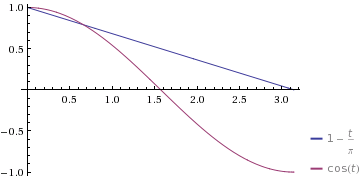
\includegraphics[width=0.6\textwidth]{cosineLSH}
\caption{approsimazione sim. coseno}
\label{fig:cosApprox}
\end{figure} 
In figura \ref{fig:cosApprox} si può notare che per piccoli angoli (non vicini all'angolo retto),  $ 1 - \frac{\theta}{\pi}$ è una buona approssimazione per  $\cos(\theta)$. Inoltre, dall'equazione \ref{eq:probhash} si ha che 
\begin{equation}
cos(\theta(u,v))=cos((1-P[h_r(u)=h_r(v)])\pi)
\end{equation}
Grazie a questa equazione, è possibile stimare la probabilità del coseno attraverso il risultato dell'applicazione delle funzioni di hashing. Guardando con più attenzione si può notare che
\begin{equation*}
 P[h_r(u)=h_r(v)])=g1-hammingDistance(h_r(u),h_r(v))/r
\end{equation*}
In pratica, questa uguaglianza permette di passare dal problema del calcolo della similarità del coseno fra due vettori altamente dimensionali, al problema del calcolo della distanza di hamming fra due stringhe.

 Anche questa famiglia di funzioni di hashing può essere aplificata con la tecnica AND-OR precedentemente descritta.
\begin{figure}
    \centering
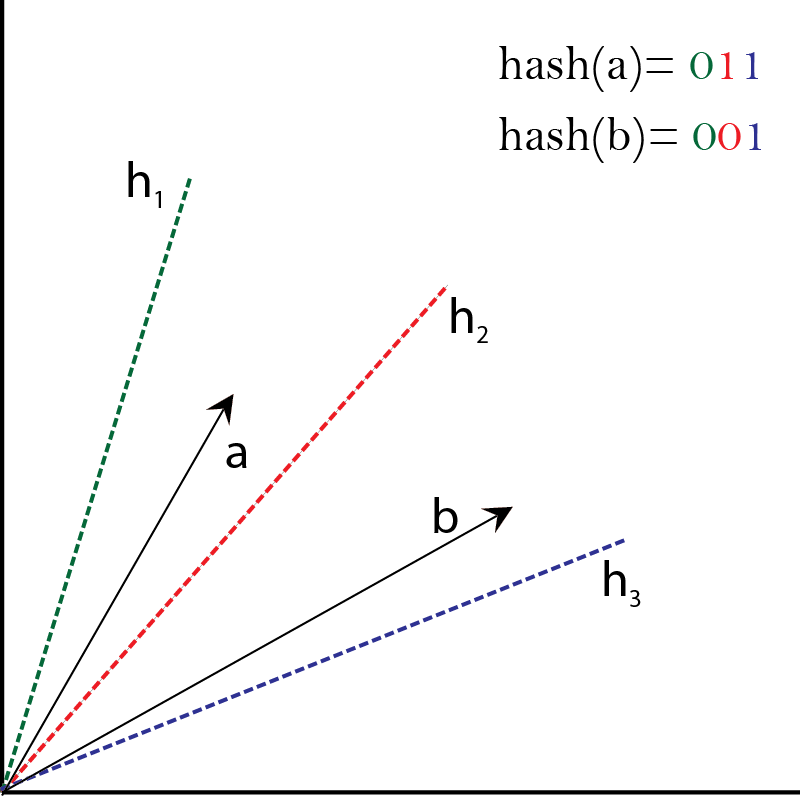
\includegraphics[width=0.5\textwidth]{hashing}
\caption{funzione di hashing}
\label{fig:hashingFunction}
\end{figure} 

 
\chapter{Sperimentazione}
\label{cap:capitolo4}
% !TEX encoding = UTF-8
% !TEX TS-program = pdflatex
% !TEX root = ../tesi.tex
% !TEX spellcheck = it-IT

%************************************************

%************************************************
\color{red}
Il sistema

-Componenti:

1. Data Cleaning;

2. NLP;

3. Information extraction and entity linking;

4. Clustering:

	- Similarità semantica;
	
    - Similarità sintatica;
   
    - Composizione;
 			

\color{black}

Dato uno stream  di tweet (ordinato temporalmente), l'obiettivo  è quello di individuare dei "topic” o “event”. In letteratura, come già descritto nel capitolo \ref{cap:capitolo2}, esistono due principali metodologie : document-pivot e feature-pivot.
In questo lavoro di tesi, è stata adottata la prima metodologia, l'obiettivo è quindi suddividere lo stream in cluster, tali che ciascuno di essi corrisponda a tutti i tweet relativi ad un \lq\lq evento\rq\rq.  
La definizione di evento utilizzata è quella utilizzata per il Topic Detection and Tracking (TDT) \cite{Allan:2002:TDT:772260} :
In seguito sono descritte in maniera più dettagliata tutte le fasi eseguite.

\begin{figure}[h]
    \centering
    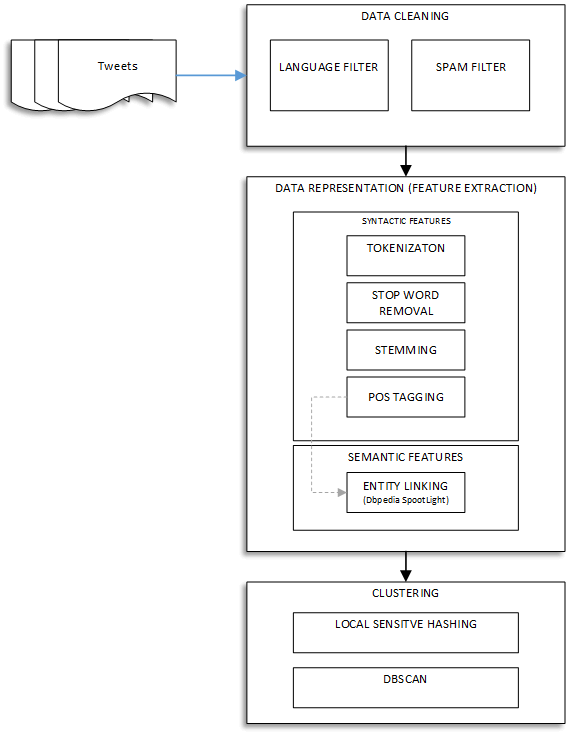
\includegraphics[width=0.6\textwidth]{diagrammaComponenti}
    \caption{Principali componenti del sistema}
    \label{fig:diagrammaComponentiSistema}
\end{figure} 


\section{Data Cleaning: Preprocessing}

Il preprocessing è uno step essenziale per qualunque task di text-mining, quando si ha a che fare con testo derivante dai social media come twitter, tale step diviene di vitale importanza a causa delle caratteristiche dei tweet. In Twitter gli utenti spesso usano slang, abbreviazione e talvolta coniano nuovi termini mai usati 
\`E dunque necessaria una fase accurata di preprocessing per il testo dei tweet prima di poter eseguire qualsiasi modellazione su di essi. 

Il primo passo in questa fase è la rimozione di quelle feature testuali legate ai tweet come:
\begin{itemize}
\item \emph{url:} dal testo sono eliminati tutti i riferimenti a url o media  
\item \emph{@-mentions:} vengono eliminate tutte le mentions ad altri utenti
\item  \emph{\#hashtag:} Per quanto riguarda gli hashtag viene solo eliminato il caratattere   \#   poiché fossero eliminati si potrebbe perdere della semantica dal testo.
Inoltre spesso nei tweet gli hashtag sono composizioni di più parole dove ciascuna parola inizia con una lettera maiuscola (camel Case), come ad esempio \#StopBombingGaza. Gli hashtag che si presentano nella forma su descritta verranno suddivisi nelle parole che di cui sono composti (\#StopBombingGaza $\rightarrow$ Stop Bombing Gaza).
\item \emph{RT:} per i retweet viene considerato il testo del tweet originale.
\end{itemize}
Per il primo passo non è necessaria alcuna fase di parsing del testo poiché tutte queste informazioni sono fornite dalle api di twitter sotto forma di dati strutturati\footnote{nell attributo entities del tweet}.

Molto spesso i tweet sono composti da keywords appartenenti a lingue diverse o contengono caratteri speciali, per tale motivo saranno eliminati tutti i non latin characters \cite{DBLP:conf/msm/BellaachiaA14} . 
 Tramite apposita espressione regolare vengono identificati ed eliminate le emoticons presenti nel testo.
 Una volta terminate queste operazioni di normalizzazione sono stati eseguite due operazioni di filtering:
 \begin{itemize}
 \item language-filtering sono stati considerati solo i tweet in lingua inglese
 utilizzando una libreria open-source scritta in java \footnote{https://code.google.com/p/language-detection/}.
 \item spam-filtering attraverso delle regole euristiche sono stati scartati quei tweet che, potenzialmente, rappresentano spam
 \end{itemize}
 
  
 
Per filtrare  quei tweet che rappresentano potenzialmente dello spam, sono state adottate delle regole empiriche:   \cite{Benevenuto10detectingspammers}
    \begin{itemize}
	\item tweet con più di tre hashtag
	\item tweet con più di due url
	\item tweet con più di tre user-mentions
	\end{itemize}
 


\section{Data Representation} 
Per poter applicare gli algorimi di machine learning è necessario rappresentare gli item attraverso vettori di feature.
I tweet saranno rappresentati come vettori, utilizzando il Vector space Model \cite{Salton:1989:ATP:77013}. 
Il Vector Space Model (VSM), in italiano Modello a Spazio Vettoriale, è una modellazione matematica per documenti testuali che si basa sull'assunzione che il significato dei documenti possa essere rappresentato dai termini che compongono il documento stesso. 
L'intero corpus di documenti, può essere quindi considerato come una matrice $A \in \mathbb{R}^{mxn}$, dove $m$  indica il numero dei termini distinti nel dizionario, $n$  il numero dei documenti 

In questo modello, ciascuna dimensione dei vettori corrisponde ad un termine distinto, e sarà diversa da zero se il termine compare nel documento: i singoli valori $a_{ij}$ della matrice rappresentano il peso
assunto dal i-esimo termine nell’j-esimo documento. Questo peso può essere assegnato in base a  diversi schemi di pesatura, ed è solitamente funzione della frequenza del termine nello specifico documento e di altri fattori, mentre assume valore 0 in assenza del
termine nel documento. Di conseguenza questi vettori sono altamente dimensionali, e molto sparsi dato che i tweet sono composti al più da 140 caratteri. 

\begin{figure}[h]
    \centering
    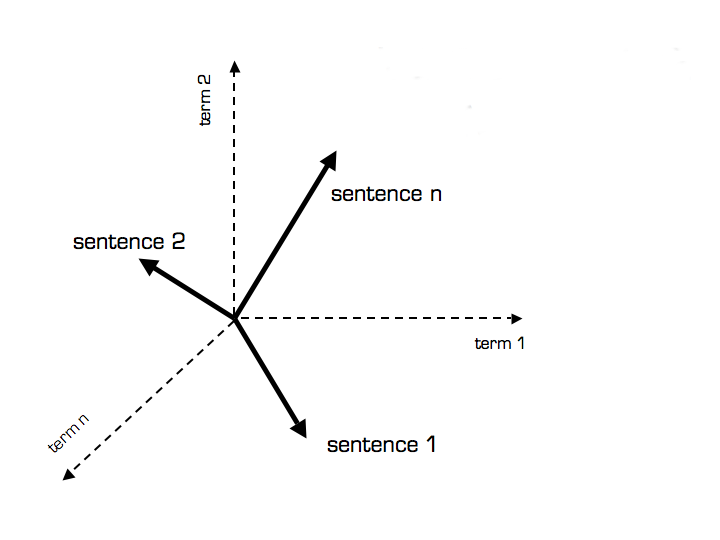
\includegraphics[width=0.6\textwidth]{vector_space}
    \caption{Esempio di documenti in uno spazio vettoriale.}
    \label{fig:dbpedia}
\end{figure}  


Il metodo di pesatura più utilizzato è quello del TF-IDF (Term Frequency-Inverse Document Frequency).
Dato una un termine  $t$, di un documento (tweet) $d$, in una collezione di documenti $D$
che è definita come  
\begin{equation}
tf-idf(t,d, D) =  tf(t,d)\cdot idf(t,D)
\end{equation}
La Term Frequency $tf(w,t)$ è dalla frequenza del termine all'interno del documento. Si presume, che un termine     ripetuto molte volte in un documento, sia molto indicativo del concetto che tale documento vuole esprimere.
Tuttavia vi sono termini che compaiono molto frequentemente in tutti i documenti (come congiunzioni. avverbi che hanno un basso potere informativo).
Per  mitigare questo effetto, viene utilizzato l'Idf che è definito come il logaritmo del rapporto fra numero totale dei documunti nel corpus, e il numero di documenti che contiene il termine $t$.
\begin{equation}
idf(t, D) =  \log \frac{|D|}{|\{d \in D: t \in d\}|}
\end{equation}
L'Inverse Document Frequency   indica la quantità di informazione di un dato termine, ovvero stabilisce se un termine è comune o meno all'interno del corpus. Più il termine è comune minore sarà la sua informazione. 
Poichè si utilizza il logaritmo, se un termine compare in tutti i documenti, il suo valore di Idf sarà pari a 0.

\subsection{Natural Language Processing}
Per poter trasformare il testo in vettori, sono state svolte delle operazioni di Natural Language Processing come:
\begin{enumerate}
\item \textbf{Tokenization}: In questa fase il testo viene suddiviso in unità atomiche dette \emph{token}
\item \textbf{Stop-Word removal}: Rimozione delle parole più comuni nel lessico
\item \textbf{Stemming}: Riduzione di ciascuna parola alla sua radice detta \emph{tema}
\item \textbf{Pos Tagging}: Ad ogni parola viene etichettata con la sua categoria lessicale (Part of Speech).
\end{enumerate}
\subsubsection{Tokenization}

La \emph{Tokenizzazione} è il primo passo di elaborazione di un sistema di Natural Language
Processing. Consiste nella separazione del flusso di caratteri che compone il testo
in input in una serie di elementi atomici detti \emph{token}. I token rappresentano le
unità minime di caratteri consecutivi e possono essere parole, spazio, simboli di
interpunzione e numeri. Sebbene questa operazione di suddivisione in token 
sembrare banale, presenta alcune problematiche. La semplice suddivisione in base allo spazio Suddividere non è sufficiente poiché in molti casi non
ci sono spazi che separano le parole dalla punteggiatura, ci sono sequenze di caratteri senza spazi al loro interno che rappresentano due distinti token (come ad esempio parole precedute da articolo con l'apostrofo, o banalmente parole virgolettate o all'interno di parentesi), esistono sequenze di caratteri. Esistono inoltre molte differenze nelle convenzioni ortografiche, ad esempio nelle date o nei numeri. 
Le tecniche per risolvere questi problemi prevedono l'uso di euristiche ed  espressioni regolari.
 
\subsubsection{Stop-Word Removal}

Le Stop Word sono parole che vengono individuate e filtrate o rimosse all'interno del processo di Natural Language Processing. Solitamente sono contenute in una lista, la stop word list, che può contenere diversi tipi di parole a seconda degli obiettivi dell'applicazione. Solitamente vengono inserite nella lista le parole a più alta frequenza e dunque meno discriminanti, di un certo linguaggio, individuabili dunque all'interno delle categorie chiuse del discorso e tra le parole a maggiore frequenza
delle altre categorie, come ad esempio verbi ausiliari o parole molto generiche. In questo lavoro è stata utilizzata una lista contenente le classiche stopword per la lingua inglese, a cui sono state aggiunte però
delle stopword specifiche per Twitter come: "Retweet","favorite","dm".
\subsubsection{Stemming}
Lo Stemming è il processo di riduzione della forma flessa o derivata di una parola alla sua radice detta \emph{tema}. 
Non è necessario che il tema corrisponda ad una valida radice morfologica, ma è utile che tutte le inflessioni o le derivazioni della parola
vengano ricondotte ad un unico tema, al fine di ridurre complessivamente lo spazio delle parole. 
 Ciò che materialmente gli algoritmi eseguono è la rimozione dei suffissi delle parole, che possono essere enclitici, ovvero essere particelle attaccate alla radice, flessioni che eseguono le declinazioni grammaticali di una parola di una certa categoria e derivazioni che cambiano categoria grammaticale o modificano il significato  

\subsubsection{Pos-Tagging}
 
Il Part of Speech Tagging, che corrisponde in italiano all'analisi grammaticale, consiste nell’associare un'etichetta che si riferisce ad una parte del discorso o categoria lessicale a ciascuna parola in una frase, basandosi sia sulla sua definizione che sul  suo contesto, ovvero la sua associazione rispetto alle parole adiacenti e correlate all’interno di una frase, di un periodo o di un paragrafo.
Le categorie lessicali in italiano sono nove, ovvero verbo, aggettivo, sostantivo,
pronome, articolo, preposizione, avverbio, interiezione e congiunzione, ma possono
variare in altri linguaggi. Cinque di queste parti si dicono variabili perché possono
mutare le loro terminazioni (articolo, nome, aggettivo, pronome, verbo) e quattro
si dicono invariabili perché non possono mutare le loro terminazione: avverbio, pre-
posizione, congiunzione e interiezione. Su di esse si basano i tagset, ovvero insiemi
di etichette che possono essere assegnati alle parole, che possono tenere in consi-
derazione solo la categoria lessicale o anche genere, numero, tempo e così via. I
più utilizzati sono il Penn Treebank   e il Multext.
Processing.
La difficoltà del passo di Part of Speech Tagging consiste nell’ambiguità dell'assegnazione di una specifica etichetta ad una parola, poiché ogni parola può essere
etichettata in diversi modi, potendo essa appartenere a diverse categorie lessicali in base al contesto in cui compare 
Gli algoritmi utilizzati per il Part of Speech Tagging sono principalmente di due
categorie:
\begin{enumerate}
\item \textbf{Basati su regole}  di trasformazione, che impostano le etichette più probabili
per le parole ambigue e successivamente applicano una serie di trasformazioni
apprese da un dataset etichettato per raffinarne i risultati 
\item \textbf{Stocastici} la maggior parte basati su Hidden Markov Model,
che, dopo aver etichettato le parole certe, massimizzano la probabilità che unasequenza di parole abbia una determinata sequenza di etichette utilizzando l'algoritmo di Viterbi \cite{Ryan:1993:VA:901051}.
\end{enumerate}
\end{enumerate}

\subsubsection{Entity Linking} 


 



Il testo del tweet verrà rappresentato con un boosted tf-idf vector utilizzando Apache-lucene\footnote{\href{https://lucene.apache.org/core/}{https://lucene.apache.org/core/}}. 
A partire dal testo dei tweet ripulito, sono state effettuati ulteriori step di nlp come :
\begin{itemize}
\item stop word removal
\item pos tagging (tramite lo stanford pos tagger addestrato su un modello  creato a partire da tweet
\item stemming (o lemmtization)
\end{itemize}
Poich\`e si analizza uno stream di tweet in maniera incrementale è necessario che anche lo schema di pesatura tf-idf sia incrementale ovvero le document-frequencies per una word $w$ variano nel tempo. 

Il peso di una word $w$ di un tweet avente tempo $t$ è dato da:
\begin{equation}
tf-idf_w=tf(w)\ log\frac{N_t}{df_t(w)}boost(w)
\end{equation}
Dove $N_t$ è il numero di tweet al tempo $t$.
Risulta fondamentale assegnare un boost a determinate word poiché, a causa della natura dei tweet (max 140 caratteri), il $tf$ di ciascuna keyword è solitamente pari a 1.  


\begin{equation*}
boost(w):=\begin{cases}
2.0 & \text{se $w$ è un hashtag, on un Proper Nooun}\\
1& \text{altrimenti.}
\end{cases}
\end{equation*}
Solitamente uh hashtag ha un alto potere informativo all’interno di un tweet, nel lavoro di  Phuvipadawat \cite{Phuvipadawat:2010:BND:1913791.1913911}  il boost maggiore per i poper-noun ha prodotto risultati migliori.

\newpage
\section{Semantic Annotation}
Tramite Dbpedia-Spootlight \cite{isem2013daiber} è possibile annotare automaticamente il testo dei tweet con DBpedia URIs.  Ciò permette di arricchire la rappresentazione testuale andando a lenire i classici problemi di ambiguità del linguaggio naturale come polisemia e sinonimia.  
Annotare il testo con DBpedia URis permette di sfruttare la base di conoscenza di DBpedia per poter determinare la correlazione semantica fra due termini. 
Il progetto DBpedia \cite{DBLP:conf/semweb/AuerBKLCI07} oltre a organizzare in maniera strutturata le informazioni di Wikipedia, le collega ad ulteriori open-datasets come: US Census, Geonames, MusicBrainz, the DBLP bibliography, WordNet, Cyc, tramite RDF links come mostrato in figura \ref{fig:dbpedia}  
\begin{figure}[h]
    \centering
    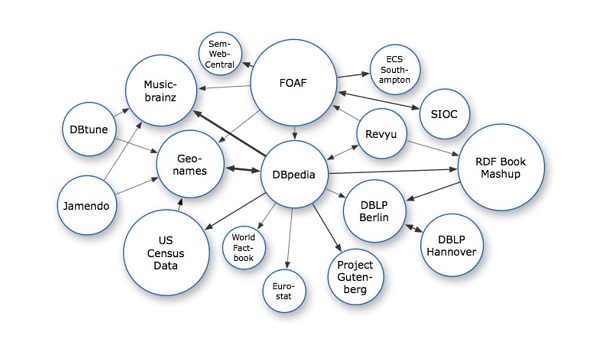
\includegraphics[width=0.6\textwidth]{dbpedia}
    \caption{Datsets interconnessi a DBpedia.}
    \label{fig:dbpedia}
\end{figure}  

Avendo due risorse DBpedia è possibile definire una funzione di distanza, che sfrutti la base di conoscenza di DBpedia. \`E stata definita  una funzione di distanza \emph{Dbpedia Semantic Distance DSD}, che impiega sia DBpedia che il dataset geografico Geonames per risorse di tipo geografico, come segue:
\begin{equation} \label{eq:dbpedia_semantic_distance}
DSD(a,b):=\begin{cases}
GeoDist(a,b) & \text{se $type(a)=location \land type(b)=location$  ,}\\
NDD(a,b) & \text{altrimenti}\\
\end{cases}
\end{equation}
Dove $DSD(a,b) \in [0,1]$,
Milne e Witten \cite{Milne08aneffective} hanno utilizzato gli hyperlink delle pagine Wikipedia per poter definire la correlazione fra due articoli wikipedia (e quindi due risorse dbpedia): date due risorse $a,b$, possiamo definire una \emph{Normalized DBpedia Distance (NDD)} come segue:
\begin{equation} \label{eq:normalized_dbpedia_distance}
NDD(a,b):=\begin{cases}
\frac{\log(max\{|A|,|B|\})-log( |A \cap B|\})}{log(N)-\log(min\{|A|,|B|\})} & \text{se $A \cap B \neq \emptyset $  ,}\\
1 & \text{altrimenti}\\
\end{cases}
\end{equation}
 $A$ e $B$  sono gli insiemi delle risorse DBpedia che hanno un link rispettivamente verso $a$ e $b$, mentre $N$ è il numero totale di risorse in DBpedia. Questa distanza varia nell'intervallo [0,1] dove 1 sta ad indicare che non vi è nessuna correlazione fra i due concetti, mentre 0 indica che i due concetti hanno lo stesso significato. L'idea alla base, è che due risorse saranno simili se esiste una terza che ha un link verso entrambe.
 
 
\section{Clustering}
L'algoritmo di clustering utilizzato è  Dbscan poiché può gestire bene il rumore e non necessita di parametri come il numero di cluster a priori. La distanza utilizzata si basa sia sulla rappresentazione tf-idf del tweet sia sui DBpedia URIs estratti :
\begin{equation}
dist(a,b)=1- timeSim(a,b)\,\frac{textSim(a,b)+semanticSim(a,b)}{2}
\end{equation}
La similarità testuale è data dalla similarità del coseno fra i vettori tf-idf dei due tweet:
\begin{equation*}
textSim(a,b)=\frac{v_a \cdot  v_b}{||v_a||\:||v_b||}
\end{equation*}
 Anche il tempo di creazione dei tweet verrà preso in considerazione per valutarne la distanza, poiché anche se due tweet avessero un testo molto simile es \emph{“tonight  flashmob in central park”}, ma fossero pubblicati ad un mese di distanza, è molto inverosimile che si riferiscano al medesimo evento. Per tale ragione, è stata definita una similarità temporale  \footnote{d$_a$=\#days from the epoch of tweet $a$}
\begin{equation*} 
timeSim(a,b):=\begin{cases}
1-\frac{|d_a-d_b|}{31} & \text{se $|d_a-d_b|<31 $  ,}\\
0 & \text{altrimenti}\\
\end{cases}
\end{equation*}
Ad un tweet, tramite il processo di annotazione semantica, possono essere associate una nessuna o più risorse DBpedia,la distanza semantica sarà data dalla distanza degli insiemi di risorse associati ai due tweet valutata secondo la distanza definita in precedenza per le risorse DBpedia\ref{eq:dbpedia_semantic_distance}. La similarità fra un elemento $x$ e un insieme $Y$ è data da:
\begin{equation*}
	sim(x,Y)=sup\{1-DSD(x,y)\:| y\in Y \}
\end{equation*}

Dati due insiemi di risorse DBpedia $D_a,D_b$ la similarità fra i due insiemi sarà definita come: 
\begin{equation}
sim(D_a,D_b)=\frac{\sum\limits_{x \in D_a} sim(x,D_b)  }{|D_a|} 
\end{equation}

Questa funzione di similarità non è simmetrica,\footnote{se $D_a\subseteq D_b\Rightarrow sim(D_a,D_b)\neq sim(D_b,D_a) $}
Per ottenere una funzione simmetrica è sufficiente definirla come: 
\begin{equation*} 
semanticSim(a,b):= 
\begin{cases}
\frac{sim(D_a,D_b)+sim(D_b,D_a)}{2} & \text{se $D_a,D_b\neq \emptyset$ }\\
1& \text{altrimenti.}

\end{cases}
\end{equation*}
Se ad uno dei due tweet non è associata nessuna risorsa, la similarità semantica sarà pari ad uno, quindi la loro similarità sarà valutata  solo in base alla loro rappresentazione testuale.
Utilizzare una similarità semantica serve ad attenuare il problema della “fragmentation” di cui sono affetti i metodi document-pivot, ovvero utilizzando solo la similarità testuale molti eventi possono essere erroneamente suddivisi in più cluster.  Inoltre Petkos e Papadopoulus \cite{DBLP:conf/www/PetkosPK14}  hanno constato che se due tweet condividono uno stesso URL, o  un tweet e in reply all’altro, allora si riferiscono allo stesso topic/evento.
 
\begin{figure}
    \centering
    \begin{subfigure}[b]{0.45\textwidth}
        \centering
        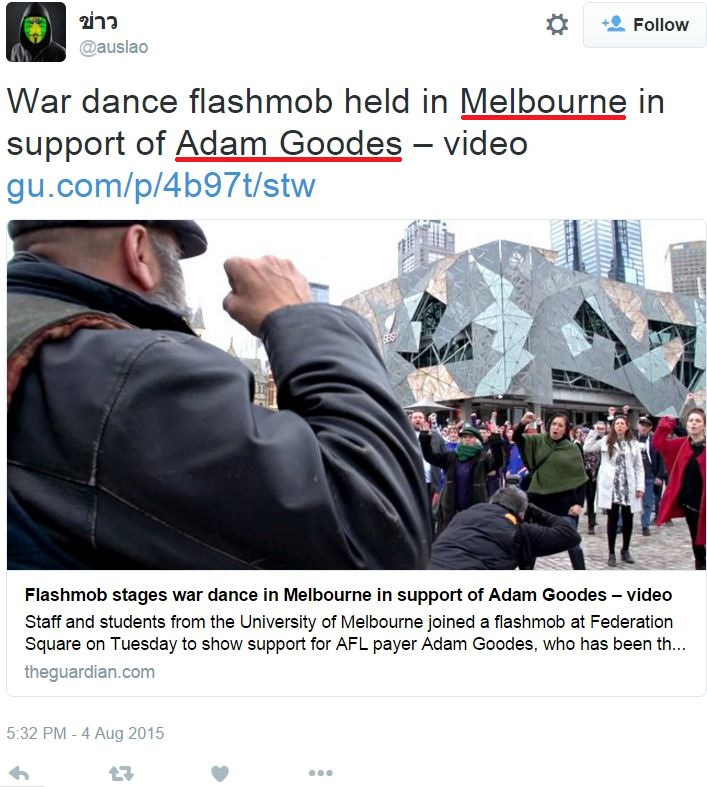
\includegraphics[width=\textwidth]{tweetA}
        \caption{}
        \label{fig:tweeta}
    \end{subfigure}
    \hfill
    \begin{subfigure}[b]{0.45\textwidth}
        \centering
        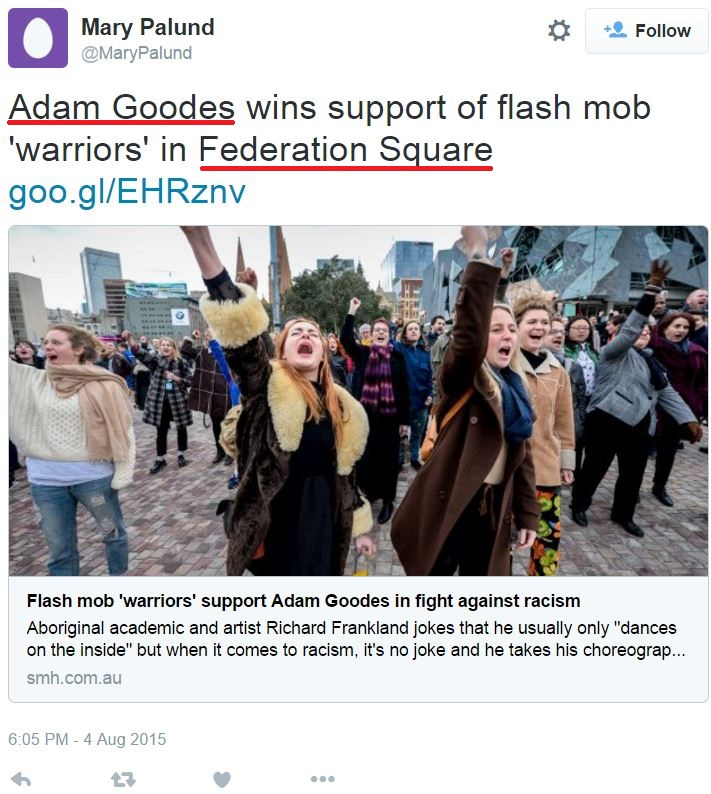
\includegraphics[width=\textwidth]{tweetB}
       \caption{}
        \label{fig:tweetb}
    \end{subfigure}
    \hfill
    
    \caption{Due tweet appartenti allo stesso cluster}
    \label{fig:twotweets}
\end{figure} 
Si considerino i tweet $a,b$ in figura \ref{fig:twotweets}:

\begin{itemize}
\item $textSim(a,b)=0.46$ 
\item $timeSim(a,b)=1.0$ i tweet sono stati pubblicati entrambi il 4/8/2015
\item $semanticSim(a,b):=\frac{sim(D_a,D_b)+sim(D_b,D_a)}{2} $



  $D_a=$\{ \textless\href{http://dbpedia.org/resource/Melbourne}{Melbourne}\textgreater, \textless\href{http://dbpedia.org/resource/Adam_Goodes}{Adam Goodes}\textgreater\}
  
  $D_b=$\{ \textless\href{http://dbpedia.org/resource/Adam_Goodes}{Adam Goodes}\textgreater, \textless\href{http://dbpedia.org/resource/Federation_Square}{Federation Square}\textgreater\}
  
\begin{align*}
 NSD(Melbourne,Adam Goodes)&=NDD(Melbourne,Adam Goodes)\\
 &= \frac{\log(max\{|A|,|B|\})-log(|A \cap B|)}{N-\log(min\{|A|,|B|\})}\\
 &= \frac{\log(643)-log(10)}{N-\log(138)}=0.367  
\end{align*} 
\begin{align*}
 NSD(Melbourne,Federation Square)&=\\
 =GeoDist(Melbourne,Federation Square)&=\\
 =CoordDist(Melbourne,Federation Square) &=0 \: \text{(poichè la distanza in km è 0.8)}
\end{align*}  
\begin{align*}
 NSD(Adam Goodes,Federation Square)=&\\
 NDD(Adam Goodes,Federation Square)&=1 \: \text{poichè} \: A \cap B=\emptyset
\end{align*} 

\begin{align*}
 sim(Melbourne,D_b)&=sup\{1-DSD(Melbourne,y)\:| y\in D_b \}\\
	&=sup\{(1-DSD(Melbourne,Adam Goodes)),\\
	&\:\:\:\:(1-DSD(Melbourne,Federation Square))\}\\
	&=sup\{(1-0.367),(1-0)\}=1	\\	  
 sim(Adam Goodes,D_b)&=sup\{1-DSD(Adam Goodes,y)\:| y\in D_b \}\\
	&=sup\{(1-DSD(Adam Goodes,Adam Goodes)),\\
	&\:\:\:\:(1-DSD(Adam Goodes,Federation Square))\}\\
	&=sup\{(1-0),(1-1)\}=1\\		 
sim(D_a,D_b) &=\frac{1+1}{2}=1 ,\: sim(D_b,D_a) :=\frac{1+1}{2}=1\\
&\implies semanticSim(a,b)=1
\end{align*}
\end{itemize} 
 \begin{align*}
dist(a,b)&=1- timeSim(a,b)\,\frac{textSim(a,b)+semanticSim(a,b)}{2}\\
&=1-\frac{0.46+1}{2}=0.269
\end{align*}

Se invece, $SemanticSim$ fosse definita come la media delle distanze fra tutte le possibili coppie fra i due insiemi avremmo: 

\begin{align*}
	semanticSim(a,b)&=\frac{\sum\limits_{x \in D_a} \sum\limits_{x \in D_b}  (1-NSD(x,y))}{|D_a||D_b|}=\\
	&=\frac{(1-0.36)+(1-0)+(1-0)+(1-1)}{4}=0.73
\end{align*}


%% !TEX encoding = UTF-8
% !TEX TS-program = pdflatex
% !TEX root = ../Tesi.tex
% !TEX spellcheck = it-IT

%************************************************
\chapter{Ipsum}
\label{cap:ipsum}
%************************************************


Lorem ipsum dolor sit amet, consectetuer adipiscing elit. Nam dui ligula, fringilla a, euismod sodales, sollicitudin vel, wisi. Morbi auctor lorem non justo. Nam lacus libero, pretium at, lobortis vitae, ultricies et, tellus.
\begin{description}
\item[Lorem ipsum dolor] sit amet, consectetuer adipiscing elit. Ut purus elit, vestibulum ut, placerat ac $\lim_{n \to \infty}\sum_{k=1}^n \frac{1}{k^2}= \frac{\pi^2}{6}$.
\item[Mauris ut leo.]
Cras viverra metus rhoncus sem. Nulla et lectus vestibulum urna fringilla ultrices. Phasellus eu tellus sit amet tortor gravida placerat.
\[
\lim_{n \to \infty}\sum_{k=1}^n \frac{1}{k^2}= \frac{\pi^2}{6}.
\]
\end{description}

Nulla malesuada porttitor diam. Donec felis erat, congue non, volutpat at, tincidunt tristique, libero. Vivamus viverra fermentum felis.
\begin{equation}
\label{eq:euler}
e^{i\pi}+1=0.
\end{equation}
Dalla formula~\eqref{eq:euler} 
si deduce che\dots






\section{Nozioni basilari}

\subsection{Insiemi numerici}

Donec nonummy pellentesque ante. Phasellus adipiscing semper elit.
\begin{equation}
x^2 \geq 0 \quad
\forall x \in \mathbb{R}.
\end{equation}


\subsection{Le matrici}

\lipsum[2]
\begin{equation}
A=
\begin{bmatrix}
x_{11} & x_{12} & \dots \\
x_{21} & x_{22} & \dots \\
\vdots & \vdots & \ddots
\end{bmatrix}
\end{equation}



\section{Formule fuori corpo}

Proin fermentum massa ac quam. Sed diam turpis, molestie vitae, placerat a, molestie nec, leo. Maecenas lacinia. Nam ipsum ligula, eleifend at, accumsan nec, suscipit a, ipsum. 


\subsection{Una formula spezzata con allineamento}

\lipsum[2]
\begin{equation} 
\begin{split} 
a &= b+c-d \\ 
  &= e-f \\ 
  &= g+h \\ 
  &= i. 
\end{split} 
\end{equation}

 
\subsection{Casi}

\lipsum[3]
\begin{equation}
f(n):=
\begin{cases} 
2n+1, & \text{con $n$ dispari,} \\ 
n/2,  & \text{con $n$ pari.} 
\end{cases} 
\end{equation}



\section{Enunciati e dimostrazioni}

Nunc eleifend consequat lorem. Sed lacinia nulla vitae enim. Pellentesque tincidunt purus vel magna. Integer non enim. Praesent euismod nunc eu purus.
\begin{definizione}[di Gauss] 
Un \emph{matematico} trova ovvio che
$\int_{-\infty}^{+\infty}
e^{-x^2}\,dx=\sqrt{\pi}$. 
\end{definizione} 
\begin{teorema} 
I matematici, se ce ne sono, sono molto rari.
\end{teorema} 

\lipsum[2]

\begin{teorema}[di Pitagora]
La somma dei quadrati costruiti sui cateti uguaglia il quadrato costruito sull'ipotenusa.
\end{teorema}
La dimostrazione viene lasciata per esercizio.

Donec bibendum quam in tellus. Nullam cursus pulvinar lectus. Donec et mi. Nam vulputate metus eu enim. Vestibulum pellentesque felis eu massa.
\begin{teorema}[Sorpresa]
Si ha che $\log(-1)^2=2\log(-1)$.
\end{teorema} 
\begin{proof} 
Si ha che $\log(1)^2 = 2\log(1)$.
Ma si ha anche che $\log(-1)^2=\log(1)=0$.
Quindi $2\log(-1)=0$, da cui la tesi.
\end{proof}
Viene un quadratino a fine dimostrazione.
\begin{legge}
\label{lex:capo}
Il capo ha ragione.
\end{legge}
\begin{decreto}[Aggiornamento alla legge~\ref{lex:capo}]
Il capo ha \emph{sempre} ragione.
\end{decreto}
\begin{legge}
Se il capo ha torto, vedere la 
legge~\ref{lex:capo}.
\end{legge}


Nam dui ligula, fringilla a, euismod sodales, sollicitudin vel, wisi. Morbi auctor lorem non justo. Nam lacus libero, pretium at, lobortis vitae, ultricies et, tellus.
\begin{murphy}
Cras nec ante. Pellentesque a nulla. Cum sociis natoque penatibus et magnis dis parturient montes, nascetur ridiculus mus. Aliquam tincidunt urna.
\end{murphy}

%\appendix
%\input{Capitoli/Dolor}
% *****************************************************************
% Materiale finale
%******************************************************************
%% !TEX encoding = UTF-8
% !TEX TS-program = pdflatex
% !TEX root = ../Tesi.tex
% !TEX spellcheck = it-IT

%*******************************************************
% Introduzione
%*******************************************************
In questo lavoro di tesi è stata trattata la problematica della sicurezza, evidenziando l'importanza che essa riveste dal punto di vista sociale e le difficoltà sociali e tecniche incontrate nella realizzazione di alcuni progetti.
La trattazione effettuata, incentrata sull'estrazione di entità nominali da documenti testuali e sulla predizione ed evoluzione delle categorie criminali nel tempo, non pretende di essere esaustiva, ma piuttosto un punto di partenza per ulteriori sviluppi, sia teorici che sperimentali. 

Il sistema TB-CREDIS è stato esteso per permettere l'estrazione dei perpetratori di un crimine all'interno di documenti più o meno segretati, che possono spaziare da articoli giornalistici a report investigativi, e predire le evoluzioni dei criminali, relativamente alle loro attività, in quegli intervalli temporali per cui non si possiede alcun documento associato al soggetto in esame relativo a tal periodo. L'alta modularità del sistema ha permesso inoltre la facile integrazione della componente di interfaccia utente: l' utente può caricare un nuovo criminale nella collezione di dati, effettuare le operazioni di predizione e visualizzare graficamente i risultati prodotti e le evoluzioni del criminale sotto analisi nel tempo.

I risultati sperimentali prodotti si sono rivelati all'altezza delle aspettative e incentivano a proseguire gli studi in questa direzione in modo da individuare nuove tecniche che permettano di migliorare i risultati raggiunti in termini di tempi di elaborazione e di qualità. 
In particolare la componente di estrazione delle entità perpetratrici può essere estesa con nuove euristiche per permettere di estrarre le entità nominali da quei pattern ad oggi non considerati, o estrarre nuove entità quali nomi di possibili vittime, luoghi, proprietà private e tutto ciò che possa rivelarsi utile alle attività investigative. 
Per la componente di predizione possibili sviluppi futuri potrebbero riguardate l'analisi e individuazione dei documenti relativi allo stesso reato, commesso da un criminale, in modo da evitare che reati più ``documentati'' abbiano più importanza di altri reati commessi nel calcolo della posizione semantica del criminale stesso.
\bibliographystyle{plain}
\bibliography{bib}                % database di biblatex 

\end{document}